\documentclass[journal]{IEEEtran}
\usepackage{multirow}
% *** CITATION PACKAGES ***
\usepackage[utf8]{inputenc}


\usepackage{cite}
\usepackage{graphicx}
\usepackage{booktabs}
\usepackage{textalpha}
\usepackage{newtxtext}
\usepackage{newtxmath}
\usepackage{url}
\usepackage{enumitem}
\usepackage{tikz}
\usetikzlibrary{arrows.meta, positioning}



\ifCLASSINFOpdf
\else
\fi

% *** MATH PACKAGES ***
%
\usepackage{amsmath}
\let\Bbbk\relax
\usepackage{amssymb}
\let\openbox\relax
\usepackage{amsthm}
\usepackage{thmtools}

\usepackage{listings}
\lstdefinelanguage{turtle}{
    morekeywords={a, prefix, base},
    sensitive=true,
    morecomment=[l]{\#},
    morestring=[b]",
}


\newtheorem{definition}{Definition}
\newtheorem{proposition}[definition]{Proposition}
\newtheorem{remark}[definition]{Remark}

\hyphenation{op-tical net-works semi-conduc-tor}

\begin{document}

\title{Resolving Semantic Conflicts in Decentralized E-Health Governance Using Zero-Knowledge Proofs}
%
%
% author names and IEEE memberships
% note positions of commas and nonbreaking spaces ( ~ ) LaTeX will not break
% a structure at a ~ so this keeps an author's name from being broken across
% two lines.
% use \thanks{} to gain access to the first footnote area
% a separate \thanks must be used for each paragraph as LaTeX2e's \thanks
% was not built to handle multiple paragraphs
%

\author{
    Aleksandr Kormiltsyn,
    Chibuzor Udokwu,
    and~Alex Norta,~\IEEEmembership{Senior Member, IEEE}%
    \thanks{
        Aleksandr Kormiltsyn is with the Department of Software Science,
        Tallinn University of Technology, Akadeemia tee 15A, 12816 Tallinn, Estonia
        (e-mail: aleksandr.kormiltson@taltech.ee).
    }%
    \thanks{
        Chibuzor Udokwu is with the IMC University of Applied Sciences Krems,
        Alauntalstrasse 96, 3500 Krems, Austria.
    }%
    \thanks{
        Alex Norta is with Tallinn University, Tallinn, Estonia;
        Department of Informatics, University of Pretoria, South Africa, Dymaxion O{\"U}, Tallinn, Estonia; and Nortadesyco.xyz
        (e-mail: alex.norta.phd@ieee.org).
    }%
}


% note the % following the last \IEEEmembership and also \thanks - 
% these prevent an unwanted space from occurring between the last author name
% and the end of the author line. i.e., if you had this:
% 
% \author{....lastname \thanks{...} \thanks{...} }
%                     ^------------^------------^----Do not want these spaces!
%
% a space would be appended to the last name and could cause every name on that
% line to be shifted left slightly. This is one of those "LaTeX things". For
% instance, "\textbf{A} \textbf{B}" will typeset as "A B" not "AB". To get
% "AB" then you have to do: "\textbf{A}\textbf{B}"
% \thanks is no different in this regard, so shield the last } of each \thanks
% that ends a line with a % and do not let a space in before the next \thanks.
% Spaces after \IEEEmembership other than the last one are OK (and needed) as
% you are supposed to have spaces between the names. For what it is worth,
% this is a minor point as most people would not even notice if the said evil
% space somehow managed to creep in.

% The paper headers

% The only time the second header will appear is for the odd numbered pages
% after the title page when using the twoside option.
% 
% *** Note that you probably will NOT want to include the author's ***
% *** name in the headers of peer review papers.                   ***
% You can use \ifCLASSOPTIONpeerreview for conditional compilation here if
% you desire.




% If you want to put a publisher's ID mark on the page you can do it like
% this:
%\IEEEpubid{0000--0000/00\$00.00~\copyright~2015 IEEE}
% Remember, if you use this you must call \IEEEpubidadjcol in the second
% column for its text to clear the IEEEpubid mark.



% use for special paper notices
%\IEEEspecialpapernotice{(Invited Paper)}




% make the title area
\maketitle

% As a general rule, do not put math, special symbols or citations
% in the abstract or keywords.
\begin{abstract}
% What is the paper about?
Building on our previous work on requirements and ontologies for decentralized governance in personalized e-health, we address semantic conflicts that arise when heterogeneous healthcare organizations represent and interpret shared clinical data in decentralized workflows. To support verifiable decision-making without revealing sensitive information, we introduce a semantic consensus framework grounded in model-theoretic semantics that provides a formal basis for evaluating the validity of clinical and policy statements and for attesting these outcomes through privacy-preserving zero-knowledge proofs (ZKPs).
% What is the state of the art?
Consensus mechanisms (e.g., PoW, PoS, PBFT) enable agreement on system state, while ontology-based approaches support semantic interoperability. ZKPs enable privacy-preserving verification of computations and protocol-level compliance.
% What is the gap in the state of the art?
However, no existing approach jointly resolves semantic conflicts 
arising from heterogeneous medical terminologies and data representations while preserving data privacy in decentralized 
governance workflows.
% What is the solution?
To address this gap, we propose a semantic consensus framework that separates semantic interpretation, cryptographic verification, and governance acceptance through a layered architecture. Semantic validity conditions are evaluated off-chain over a Decentralized Knowledge Graph (DKG) and attested using zero-knowledge Succinct Non-interactive ARguments of Knowledge (zk-SNARK) proofs without revealing underlying medical data.
% Why is the solution good/better than other solutions?
The governance layer, implemented as a Decentralized Autonomous Organization (DAO), verifies these proofs and reaches agreement on semantic outcomes rather than on raw data, enabling privacy-preserving coordination across heterogeneous healthcare systems.
\end{abstract}


% Note that keywords are not normally used for peerreview papers.
\begin{IEEEkeywords}
Semantic consensus, decentralized governance, e-health systems, 
zero-knowledge proofs, semantic interoperability, 
privacy-preserving verification.
\end{IEEEkeywords}

% For peer review papers, you can put extra information on the cover
% page as needed:
% \ifCLASSOPTIONpeerreview
% \begin{center} \bfseries EDICS Category: 3-BBND \end{center}
% \fi
%
% For peerreview papers, this IEEEtran command inserts a page break and
% creates the second title. It will be ignored for other modes.
\IEEEpeerreviewmaketitle

\section{Introduction}
\IEEEPARstart{H}{ealthcare} data breaches have reached unprecedented levels, with profound implications for patient privacy, organizational costs, and public trust. In 2024 alone, 735 large-scale breaches affecting more than 276 million individuals were reported in the United States, representing the worst year on record for healthcare data security~\cite{HIPAAJournal2024Statistics, HIPAAJournal2024Largest}. Incidents such as the Change Healthcare ransomware attack demonstrate the scale and systemic impact of these vulnerabilities~\cite{HealthcareIT2024}. While these developments highlight the need for stronger privacy-preserving infrastructures, inter-organizational healthcare collaboration also introduces semantic challenges, as different institutions may represent and interpret shared data and clinical concepts in different ways.

The financial consequences of healthcare data breaches are equally severe. According to IBM's 2024 Cost of a Data Breach Report, healthcare organizations face the highest average breach cost across all industries, reaching \$9.77 million per incident~\cite{IBM2024Cost}. Beyond financial losses, breaches disrupt clinical operations and patient care, with many healthcare providers reporting prolonged service interruptions following major incidents~\cite{IBM2024Cost}. These challenges further complicate secure and trustworthy collaboration between healthcare organizations.

Despite the need for stronger security and privacy mechanisms, the adoption of blockchain technology in healthcare remains limited. Studies indicate that only a small fraction of healthcare organizations have implemented blockchain-based solutions due to high implementation costs, regulatory uncertainty, and integration challenges with existing Electronic Health Record (EHR) systems~\cite{Nature2025Blockchain, Healthcare2024Barriers}. These limitations highlight the need for architectures that not only address privacy concerns but also support trustworthy collaboration across heterogeneous healthcare systems.

Collaboration in inter-organizational decentralized e-health processes is complicated by privacy constraints, the sensitivity of health data, and legal regulations governing medical information. In addition, heterogeneous and partially trusted data sources introduce integrity, provenance, and semantic interpretation challenges that require verifiable reconciliation across institutions. Current blockchain solutions provide transparency, data integrity, and ownership guarantees, but they primarily ensure agreement on system state rather than on the semantic validity of clinical or governance decisions. As a result, existing blockchain-based approaches do not address governance-level trust and compliance in environments where different organizations may interpret the meaning and validity of shared healthcare data differently.

Although consensus mechanisms ensure agreement on transactions and system state in decentralized systems, they operate at the level of data ordering and do not address semantic interpretation~\cite{10075075, Nasir2024, AlAwamy2025, yakubu2024systematic}. As a result, they cannot guarantee a consistent understanding of the meaning or validity of shared data among heterogeneous participants.

Various studies are exploring blockchain-based e-health architectures and governance models~\cite{Andrew2023,elvas2023sharing,alruwaill2025hchain,Villarreal2023,jha2025blockchain}. These approaches aim to improve data security, transparency, patient control, and interoperability in healthcare systems. In parallel, standards such as HL7 FHIR are widely used to enable interoperable exchange of clinical information between healthcare systems~\cite{gazzarata2024hl7}. Although such standards facilitate structural interoperability and support applications such as Clinical Decision Support Systems (CDSS), they primarily address data representation and exchange rather than semantic agreement on the validity or meaning of clinical decisions. As a result, even when shared data conform to common standards, organizations can still interpret their meaning differently, leading to unresolved semantic conflicts in decentralized healthcare workflows.

Research~\cite{Lavin2024} identifies zero-knowledge proof (ZKP) protocols as an important mechanism to achieve privacy-preserving verification in decentralized systems. Much of the existing work focuses on improving the efficiency and scalability of ZKP constructions~\cite{xie2023advances}, including approaches that reduce verification costs through techniques such as folding-based proofs~\cite{sakwa5293078survey}. In the healthcare domain, several studies explore the use of ZKP for secure data processing and privacy-preserving communication~\cite{babu2024secure,9387630}. These approaches demonstrate how ZKP can verify computations or compliance conditions without revealing sensitive data. However, current applications of ZKP focus primarily on validating numerical computations or protocol-level properties rather than on verifying the semantic correctness of domain-specific interpretations. Consequently, integration of ZKP-based verification with semantic conflict resolution and governance-level decision-making in decentralized healthcare settings remains largely unexplored.

Despite substantial progress in decentralized consensus, blockchain-based e-health architectures, and privacy-preserving computation, current research focuses on several critical limitations:

\begin{itemize}

\item \textit{Network-layer focus without semantic interoperability:} 
Existing consensus mechanisms (PoW, PoS, PBFT) achieve agreement at the protocol level but do not address semantic conflicts arising from heterogeneous medical terminologies and interpretations (e.g., SNOMED-CT vs. local codes)~\cite{Nasir2024, AlAwamy2025}.

\item \textit{Transparency without sufficient privacy guarantees:} 
Blockchain solutions provide immutability and auditability of data, but their intrinsic transparency can expose sensitive patient information on the chain, creating challenges to comply with privacy regulations such as GDPR and HIPAA~\cite{Andrew2023, Villarreal2023}.

\item \textit{Limitations of existing privacy-preserving techniques:} 
Approaches such as Multi-Party Computation, Homomorphic 
Encryption, and Differential Privacy do not support verifiable 
semantic decision-making in asynchronous decentralized 
governance workflows~\cite{Evans2018, Gentry2009}.

\item \textit{Lack of governance-aware semantic consensus: Current systems lack formal mechanisms that enable verifiable compliance with governance-approved clinical rules (e.g., treatment protocols, ontological constraints) within decentralized decision-making processes~\cite{Angurala2025, Amin2024}}.

\item \textit{No integration of semantic truth with cryptographic verification:} 
The integration of semantic conflict resolution—grounded in formal model-theoretic semantics (e.g., Tarski's theory of truth)—with ZKP-based verification mechanisms remains largely unexplored~\cite{Lavin2024}.

\end{itemize}

These limitations make it difficult to use reliable and transparent decentralized systems to manage e-health in different organizations. This is especially true when institutions need to resolve differences in meaning and agree on clinical decisions, while still keeping data private. In this paper, the object of agreement is not a numeric aggregation result, but the acceptance of semantic statements arising in cross-organizational e-health workflows (e.g., whether a prescription is valid under allergy and renal-function constraints). Such workflows often involve semantic conflicts, as different organizations may interpret clinical data differently. We model these statements using a domain-specific representation and evaluate their truth under a shared semantic model and governance-approved evaluation context based on model-theoretic semantics. The resulting acceptance/rejection outcome provides a verifiable basis for governance-level consensus among autonomous participants. In our design, patient-specific evidence remains off-chain and is used only as private witness input during proof generation, while the public ledger anchors governance-approved ontology and policy artifacts together with privacy-preserving commitments (e.g., hashes or Merkle roots) for auditability. This architecture enables privacy-preserving verification of governance policy compliance ensuring that a clinical statement satisfies the governance-approved rules encoded in~$T$ under zero-knowledge.

We distinguish two notions of compliance that must not be conflated:

\begin{itemize}
  \item \textbf{Compliance with governance policy} (in scope): the protocol verifies, using zk-SNARK proofs, that the evaluated statements satisfy the formal rules encoded in~$T$ and anchored in the DKG. This is the compliance claim made in the paper.
  \item \textbf{Regulatory compliance} (out of scope): adhesion to external legal frameworks such as GDPR, HIPAA, or national health data regulations, including consent management, data retention, and erasure obligations. These requirements depend on organizational processes and legal interpretation that cannot be reduced to arithmetic circuit constraints. They are handled by institutional processes and are outside the scope of the protocol.
\end{itemize}

The main contributions of this paper are as follows:
\begin{itemize}

\item We introduce a model-theoretic semantic framework, grounded in Tarski's theory of truth, for representing and evaluating clinical and governance statements in decentralized e-health workflows (Section~\ref{ss:semantic}).

\item We derive formal requirements for verifiable semantic decision-making in cross-organizational e-health environments, capturing semantic interoperability, privacy, and governance policy constraints (Section~\ref{s:rq1}).

\item We propose an architectural model that separates semantic interpretation, cryptographic verification, and governance acceptance, allowing decentralized participants to reach \emph{verifiable agreement} on the validity of semantic statements rather than on raw data (Section~\ref{s:rq2}).

\item We design a zk-SNARK-based verification pipeline that compiles semantic validity conditions into cryptographic constraints and integrates proof generation and verification into decentralized governance workflows (Section~\ref{s:rq3}).

\end{itemize}


\noindent Based on the detected gap in the state-of-the-art research, the main research question is:

\begin{description}[leftmargin=\IEEElabelindentfactor\IEEElabelindent,labelsep=0.5em, style=nextline]
\item[\textbf{Main RQ}] \textit{How can decentralized e-health workflows achieve semantic consensus on clinical statements while preserving privacy and enabling verifiable governance decisions through zero-knowledge proofs?}
\end{description}

\noindent To establish a separation of concerns, we deduce the following sub-questions:

\begin{description}[leftmargin=\IEEElabelindentfactor\IEEElabelindent,
                    labelsep=0.5em, style=nextline]
\item[\textbf{RQ1}] \textit{What are the formal requirements for privacy-preserving semantic consensus in decentralized e-health inter-organiational processes?}

\noindent The answer to this question identifies the requirements for semantic statement evaluation, interoperability, and verifiable governance acceptance in decentralized workflows.

\item[\textbf{RQ2}] \textit{What architectural and governance mechanisms enable privacy-preserving semantic verification and acceptance of clinical decisions across heterogeneous healthcare organizations?}

\noindent Answering this question specifies the architecture and governance workflow in which semantic evaluation results are anchored and verified, while ZKPs provide cryptographic evidence for private \emph{governance policy} verification.

\item[\textbf{RQ3}] \textit{What cryptographic mechanisms and circuit
constructions are required to encode semantic validity conditions into
zero-knowledge proofs while preserving privacy, correctness, binding,
and governance verifiability?}

\noindent The answer to this question defines the technical design of
the zk-SNARK-based proof construction and verification pipeline.
\end{description}

The remainder of this paper is organized as follows. Section \ref{s:related-work} analyzes related research in a similar field. Section~\ref{ss:rc} introduces the e-health running case and the necessary preliminaries. Section~\ref{s:rq1} derives the requirements for semantic consensus and conflict resolution in decentralized e-health workflows. Section~\ref{s:rq2} presents the proposed architectural and governance mechanisms that address these requirements. Section~\ref{s:rq3} describes the verification pipeline based on zk-SNARK, including witness and public inputs and its integration into the governance workflow. Section~\ref{s:eval} evaluates the proposed approach using the e-health running case with formal validation in CPN. Section~\ref{s:discussions} discusses the results, limitations, and open research directions. Finally, Section~\ref{s:conclusion} concludes the paper.

\section{Related Work}
\label{s:related-work}

Research related to this work spans three intersecting areas:
decentralized consensus mechanisms and blockchain-based governance,
privacy-preserving verification using zero-knowledge proofs in
healthcare, and semantic interoperability for heterogeneous health
data. Each area contributes essential building blocks to the problem
addressed in this paper, but none of their existing contributions
fully integrates all three concerns into a coherent governance
framework. Section~\ref{ss:consensus} discusses decentralized consensus
and blockchain governance in healthcare. Section~\ref{ss:zkp} reviews
zero-knowledge proof systems and their application to
privacy-preserving verification. Section~\ref{ss:semantic} addresses
semantic interoperability and introduces the formal model-theoretic
foundations adopted in this work. A running case consolidating the
identified gaps is presented in Section~\ref{ss:rc}.

\subsection{Decentralized Consensus and Blockchain Governance
in Healthcare}
\label{ss:consensus}

Blockchain technology has been widely adopted to address trust,
transparency, and data integrity challenges in healthcare.
A survey of blockchain architectures for healthcare systems
identifies security, scalability, and interoperability as persistent
barriers to adoption~\cite{Andrew2023}. Related work examines how
blockchain can facilitate health information sharing while maintaining
auditability~\cite{elvas2023sharing}, and a permissioned blockchain
framework for secure EHR management demonstrates practical deployment
at the institutional level~\cite{alruwaill2025hchain}. These works
collectively establish the potential of blockchain for healthcare data
management, but they operate at the level of transaction ordering and
data immutability rather than on the semantic validity of clinical
decisions derived from shared data.

Consensus mechanisms form the foundation of distributed agreement in
blockchain systems. A comprehensive treatment of consensus in data
management covers both classical commit protocols and
blockchain-specific constructions from a distributed systems
perspective~\cite{10075075}. The security implications of consensus
mechanisms for permissioned blockchain systems are analyzed
in~\cite{Nasir2024}, while hybrid consensus models that combine
on-chain and off-chain components to balance performance and trust are
introduced in~\cite{AlAwamy2025}. Security vulnerabilities in
blockchain consensus and corresponding mitigation strategies for open
challenges are surveyed in~\cite{yakubu2024systematic}. Despite this
substantial body of work, existing consensus mechanisms are designed
to achieve agreement on transaction ordering and system state. They
do not address the semantic layer: whether participating organizations
interpret the meaning and validity of shared clinical data in the same
way.

Decentralized governance through DAO structures has attracted
increasing attention as a mechanism for managing shared resources
without central authority. A survey of blockchain-based governance
models for healthcare management systems highlights the potential for
multi-stakeholder decision-making in interoperable
settings~\cite{Villarreal2023}. The transformative role of blockchain
in healthcare privacy and regulatory compliance is explored
in~\cite{Angurala2025}. An integrative review of DAO governance
models distinguishes between purely on-chain voting and hybrid
governance structures that incorporate off-chain
deliberation~\cite{cabello2024exploring}. The broader potential of
DAOs to reshape healthcare management, including transparent
governance and decentralized funding, is discussed
in~\cite{mateus2023can}. However, none of these works address how
governance decisions can be grounded in formally verifiable semantic
criteria rather than simple majority votes over raw or aggregated
data.

\subsection{Zero-Knowledge Proof Systems}
\label{ss:zkp}

Zero-knowledge proofs (ZKPs) enable the verification of constraint
satisfaction without revealing the underlying witness data. In
decentralized healthcare settings, ZKPs provide a cryptographic
mechanism to preserve privacy by verifying clinical constraints and
semantic validity conditions derived from sensitive medical data.

Several classes of ZKP systems are relevant in this context.
Specifically, zk-SNARKs provide short, non-interactive proofs with
efficient verification, making them suitable for on-chain governance
workflows. zk-STARKs avoid trusted setup assumptions and offer
post-quantum security at the cost of larger proofs. Bulletproofs
support efficient range and constraint proofs without trusted setup
but typically incur higher verification overhead for more complex
verification tasks~\cite{ouderoelink2024slr}. These trade-offs are
particularly important in governance settings, where proofs must
remain compact enough for practical verification while still encoding
semantically meaningful constraints.

Zero-knowledge proof systems have emerged as a key cryptographic
primitive for enabling verifiable computation without disclosing
sensitive information. A comprehensive survey of ZKP applications in
blockchain covers membership proofs, range proofs, and
general-purpose arithmetic circuits~\cite{Lavin2024}. Advances in ZKP
constructions with particular attention to bridging theoretical
efficiency and practical deployment are surveyed
in~\cite{xie2023advances}, while folding-based proof composition as a
scalable path toward incrementally verifiable computation is
investigated in~\cite{sakwa5293078survey}.

In the healthcare domain, ZKP systems have been applied primarily to
protect patient identity and secure data exchange. A ZKP-based
framework for privacy-preserving analytics over healthcare records
stored on blockchain is proposed in~\cite{babu2024secure}. Research
on vehicle-to-healthcare communications demonstrates how
zero-knowledge and statistical fingerprinting can protect sensitive
medical data in transit~\cite{9387630}. A ZKP-enabled blockchain
system for wearable health device data management demonstrates
measurable improvements in privacy and data integrity for
IoT-generated clinical evidence~\cite{khan2025leveraging}. The MEPCA
framework addresses on-chain EHR validation using cryptographic
commitments and HL7~FHIR compliance checks, demonstrating that
cryptographic anchoring of clinical data can support regulatory
auditability~\cite{da2025enhancing}. A combination of ZK-Rollups with
smart contracts and decentralized storage is proposed to improve
scalability for cross-institutional health data exchange, decoupling
proof generation from on-chain settlement latency~\cite{raghav2026secure}.

Privacy-preserving alternatives to ZKP, including Multi-Party
Computation (MPC) and Homomorphic Encryption (HE), have also been
applied in healthcare. A pragmatic introduction to MPC covers its
use in privacy-preserving analytics and the synchronous participation
requirements that constrain its applicability~\cite{Evans2018}. Fully
homomorphic encryption was established as a theoretical foundation for
computation over encrypted data in~\cite{Gentry2009}. The balance
between patient privacy and regulatory compliance in PHI-sharing
scenarios is examined in~\cite{Amin2024}. While powerful, MPC
requires synchronous participation from all parties---a constraint
incompatible with asynchronous clinical workflows---and HE introduces
substantial computational overhead for general-purpose arithmetic.
ZKP systems, particularly non-interactive constructions such as
Groth16-based zk-SNARKs~\cite{groth2016}, avoid both limitations by
generating compact, independently verifiable proofs off-chain.

These works establish that ZKP systems are technically viable in
healthcare settings. However, existing applications focus on proving
properties of \emph{data}---such as membership in a dataset, range
conditions on numerical values, or identity claims---rather than on
proving the semantic correctness of \emph{clinical decisions} derived
from heterogeneous ontological sources. The circuit designs in these
works encode numerical or structural constraints but do not capture
first-order logical reasoning over domain-specific medical semantics.
A survey of ZKP applications in blockchain identifies this gap,
noting that semantic verification remains an underexplored
direction~\cite{peng2024zkpblockchain}. The present work directly
addresses this limitation by encoding model-theoretic satisfaction
conditions as arithmetic constraints, enabling zero-knowledge proofs
of semantic acceptance over governance-approved clinical and policy
statements.

\subsection{Semantic Interoperability and Formal Foundations}
\label{ss:semantic}

Semantic interoperability remains one of the most persistent
challenges in cross-institutional healthcare collaboration. Standards
such as HL7~FHIR and SNOMED-CT provide frameworks for structural and
terminological consistency, but they do not guarantee that
heterogeneous organizations will interpret shared data according to
compatible semantic rules. A scoping review of HL7~FHIR resources in
digital healthcare ecosystems for chronic disease management documents
how even standards-compliant systems can produce semantically
inconsistent outcomes when organizations apply different local
policies~\cite{gazzarata2024hl7}. Research on blockchain-empowered
personal health records proposes enhancements to interoperability,
but addresses data representation rather than the semantic correctness
of clinical decisions derived from that data~\cite{jha2025blockchain}.

Knowledge graphs and ontology-based reasoning have been proposed as
tools for achieving deeper semantic integration. A framework for
encoding smart contract logic using a semantic knowledge graph derived
from HL7~FHIR concepts, compiled into deployable Solidity contracts
via an off-chain code generation pipeline, achieves structural
interoperability by ensuring that contract logic reflects the
vocabulary and relations of a shared domain
standard~\cite{van2025semantic}. This is conceptually adjacent to our
use of a Decentralized Knowledge Graph (DKG) to anchor
governance-approved ontologies and theory axioms. However, that
framework does not address semantic conflicts that arise when different
organizations apply heterogeneous terminologies or data representations
to the same clinical facts, and it does not
incorporate privacy-preserving verification mechanisms. In contrast,
the present work treats semantic conflict resolution as a first-order
concern: the framework verifies whether a clinical statement is
semantically true under a shared model and governance-approved theory,
and attests to this outcome cryptographically without revealing the
underlying patient evidence.

Formal model-theoretic semantics, particularly Tarski's theory of
truth~\cite{tarski1944semantic}, provides a rigorous foundation for
evaluating the truth of statements with respect to a model and
variable assignment. Model theory further develops these ideas and
establishes the mathematical basis for the satisfaction relation used
in this work~\cite{hodges1997shorter}. While Tarski's framework is
well established in logic and formal semantics, its application to
decentralized governance in healthcare systems---where the model is
constructed dynamically from heterogeneous and partially trusted
sources---has not previously been explored. Prior work on
cross-blockchain e-health systems motivates the need for architectures
that verify semantic correctness without relying on centralized trust
anchors~\cite{mfssia}. We adopt this framework as the formal
foundation for semantic consensus in our architecture, organized
around three complementary components introduced below.

\paragraph{$M = \langle D, I \rangle$ — static semantic model
           (the facts).}

We model shared clinical knowledge as a \emph{semantic model}:
\begin{equation}\label{eq:model}
  M = \langle D,\, I \rangle
\end{equation}
where $D$ is a typed domain comprising entities of several kinds
(patients, medications, substances, prescribers, and record
identifiers for allergies and lab observations), and $I$ is an 
interpretation function that assigns meaning to each relation 
over~$D$.

Following the model-theoretic semantics of RDF~\cite{rdf12semantics2026}
and the named-graph approach to provenance~\cite{massari2023representing},
clinical facts are represented as \emph{labeled entities}: each
record is a first-class entity in~$D$ whose attributes (subject,
clinical content, source) are expressed through
binary relations in~$I$.  For example, an allergy record~$a_1$
stating that patient~\textit{pat1} has a documented allergy to
Penicillin, recorded by hospital~$H$, is represented
as:
\begin{align*}
  & a_1 \in I(\mathit{isAllergy}) \\
  & \langle a_1,\, \mathit{pat1} \rangle \in I(\mathit{hasPatient}) \\
  & \langle a_1,\, \mathit{Penicillin} \rangle \in I(\mathit{hasSubstance}) \\
  & \langle a_1,\, H \rangle \in I(\mathit{hasSource})
\end{align*}
This structure mirrors directly the RDF-triple representation
anchored in the Decentralized Knowledge Graph (DKG), with
public commitments to entity identifiers; the full attribute
content resides off-chain with its respective custodians and is
revealed only through zero-knowledge proofs
(Section~\ref{s:rq3}).

A key consequence of the labeled-fact representation is that
independent observations of the same clinical condition---for
example, an allergy recorded by a hospital and separately
confirmed by a laboratory---correspond to \emph{distinct}
entities~$a_1, a_2 \in I(\mathit{isAllergy})$, each with its own
provenance.  Both facts coexist in~$M$, reflecting the
decentralized reality that multiple independent sources may
report on the same clinical condition.

\paragraph{$T = \{\alpha_1, \ldots, \alpha_n\}$ — governance-approved
           theory (the rules).}

Clinical and governance rules collected in a governance-approved
\emph{theory}:
\begin{equation}\label{eq:theory}
  T = \{\alpha_1,\, \alpha_2,\, \ldots,\, \alpha_n\}
\end{equation}
A model $M$ is \emph{admissible} if it satisfies every axiom
in~$T$, written $M \models T$. The theory~$T$ is anchored in
the Decentralized Knowledge Graph (DKG), ensuring that all
participants evaluate statements against the same set of
governance-approved rules.

Four classes of axioms are distinguished, each addressing a
distinct form of semantic heterogeneity encountered in
cross-organizational e-health workflows:

\begin{itemize}
  \item \textit{Ontological hierarchies} capture subsumption
    relations among clinical concepts, such as
    $\mathrm{Penicillin} \sqsubseteq \mathrm{\beta{-}lactam}$.
  \item \textit{Inference rules} propagate clinical implications
    along hierarchical and relational structure, such as
    ``allergy to a class implies contraindication for class
    members''.
  \item \textit{Terminology bridges} align equivalent predicates
    expressed in heterogeneous coding systems, e.g.\ mapping a
    SNOMED~CT allergy predicate to a laboratory's local coding.
  \item \textit{Numerical bridges} relate clinical values
    obtained by different formulas or in different units, such
    as converting a Cockcroft-Gault creatinine clearance in
    $\mathrm{mL/min}$ to an eGFR value in
    $\mathrm{mL/min/1.73m^2}$ computed via CKD-EPI, so that
    independent laboratory observations can be compared against
    a single governance-approved clinical threshold.
     \item \textit{Clinical policy axioms} encode governance-approved
    threshold conditions on medications, e.g.
    $\mathrm{Pol}(\mathrm{Metformin}, \mathrm{eGFR}, \geq, 30)$
    requires the patient's eGFR to be at least
    $30\,\mathrm{mL/min/1.73m^2}$.
\end{itemize}

In our running case, for example, the hospital's clinical policy
requires an eGFR threshold computed via CKD-EPI, whereas an
independent laboratory reports creatinine clearance computed via
the Cockcroft-Gault formula. Without~$T$, the two measurements
describe the same patient's renal function but cannot be jointly
evaluated against the policy threshold; the numerical bridge
axiom in~$T$ reconciles the representations, so that different
laboratories contribute comparable evidence to the same clinical
decision.

\paragraph{$\Gamma = \langle \mathit{cred}, \mathit{refs},
           \mathit{t_{req}} \rangle$ — dynamic evaluation context
           (the request).}

In classical first-order semantics, truth of a statement depends
only on the model. In decentralized cross-organizational
workflows, however, evaluating a clinical statement additionally
requires reasoning about \emph{the request itself}: who initiated
it, which specific facts in~$M$ it relies upon, and when it was
issued. These concerns are not properties of the world, and
therefore do not belong to~$M$; nor are they rules of clinical
practice belonging to~$T$. They are epistemic metadata of the
current evaluation attempt, and we collect them in an
\emph{evaluation context}:
\begin{equation}\label{eq:ctx}
  \Gamma = \langle \mathit{cred},\, \mathit{refs},\,
                   \mathit{t_{req}} \rangle
\end{equation}
Each component of~$\Gamma$ carries a distinct kind of
request-specific information:
\begin{itemize}
\item $\mathit{cred}$ is the \emph{credential} presented by
    the initiator of the request. It is issued by a
    governance-approved authority and registered in the
    governance-approved credential registry. The credential
    is verified for validity without disclosing identity or
    role attributes of the credential holder.
  \item $\mathit{refs}$ is the \emph{set of record identifiers}
    in~$M$ that the request explicitly relies upon---for
    example, the allergy records and laboratory observations 
    invoked by a particular
    prescription. Referencing records explicitly, rather than
    leaving them implicit, makes the evidentiary basis of the
    request auditable and enables the patient, the governance
    layer, and external observers to trace which facts informed
    a given clinical decision.
  \item $\mathit{t_{req}}$ is the \emph{timestamp of the
    request}, recorded as the prescription issuance time.
    It is consumed downstream by operational checks such as
    the pharmacy's validity-window check at dispensing
    (Section~\ref{sec:governance-layer}).
\end{itemize}

Two properties distinguish~$\Gamma$ from the model~$M$ and the
theory~$T$. First, $\Gamma$ is \emph{dynamic}: it changes with
every evaluation instance, depending on who initiates the
request, when, and which records are invoked. Second, $\Gamma$
contains \emph{no clinical facts}: it only declares \emph{which}
facts in~$M$ the request uses, through $\mathit{refs}$. The
facts themselves---including their provenance---reside in~$M$
as labeled entities, as described above.

In our running case, the hospital's physician
$\mathit{doc_1}$ initiates a prescription request for patient
$\mathit{pat_1}$. The evaluation context carries the physician's credential, the specific record identifiers
invoked by the prescription (the patient's current allergy
record and the most recent eGFR observation), and the timestamp
of the request:
\[
  \Gamma = \langle \mathit{cred}_{\mathit{doc_1}},\,
                   \{a_2,\, l_3\},\,
                   \mathit{t_{req}}
           \rangle.
\]
The facts themselves---the allergy recorded by hospital~$H$, the
eGFR value obtained by Lab~1---reside in~$M$ with their own
provenance. $\Gamma$ does not duplicate them; it
only declares that the current request relies on them. Whether
this reliance is legitimate---whether the credential is valid,
the referenced records exist in~$M$, and their sources are
trusted---is established by
a dedicated predicate defined in Section~\ref{sec:formal-basis}.

Since all statements evaluated in the prescription workflow are
\emph{ground}---instantiated with concrete identifiers such as
a specific physician, patient, and medication---variable
assignments are fully determined and omitted throughout this
paper~\cite{hodges1997shorter}.

\paragraph{Summary of roles.}

The three components serve complementary and non-overlapping
roles:
\begin{itemize}
  \item $M = \langle D, I \rangle$ stores \emph{the facts}:
        labeled clinical records---allergies and laboratory
        observations---each
        carrying its own provenance as part of
        the record's attributes;
  \item $T$ stores \emph{the rules}: governance-approved axioms
        for interpreting and relating facts across organizational
        boundaries (ontologies, inference rules, terminology and
        numerical bridges, clinical policy thresholds);
  \item $\Gamma = \langle \mathit{cred}, \mathit{refs},
        \mathit{t_{req}} \rangle$ carries the \emph{request
        context}: the initiator's credential, explicit
        references to the records in~$M$ that the request
        relies upon, and the time of the request itself.
\end{itemize}

Semantic evaluation then combines two complementary checks: the
request context $\Gamma$ is trusted with respect to~$M$ and~$T$,
and the clinical statement~$\varphi$ is satisfied in~$M$ under
classical Tarski semantics. These are formalized as distinct
relations in Section~\ref{sec:formal-basis}.

Together, the surveyed literature reveals three persistent gaps
that the present work addresses. First, existing consensus
mechanisms operate at the transaction level and do not extend to
semantic agreement on the validity of clinical decisions. Second,
ZKP applications in healthcare focus on data properties rather
than the semantic correctness of reasoning performed over
heterogeneous ontological sources. Third, semantic
interoperability frameworks for healthcare lack cryptographic
mechanisms to verify that shared governance rules have been
correctly applied without disclosing the underlying patient
evidence. The framework proposed in this paper bridges these
gaps by introducing a semantic consensus architecture that
separates semantic interpretation, cryptographic verification,
and governance acceptance into distinct functional layers,
grounding each in a formally specified satisfaction relation,
and realizing it through a zk-SNARK proof pipeline integrated
into a DAO-governed e-health infrastructure.

\subsection{Running case}
\label{ss:rc}
We extend a running case originally developed in the TEH-BLMIC 2025 workshop to analyze semantic conflicts in inter-organizational prescription workflows in decentralized healthcare. The running case was refined through discussions with healthcare and technical experts on blockchain-enabled healthcare data management in low- and middle-income settings. The scenario involves three autonomous and decentralized entities: a public hospital, a private diagnostics laboratory, and a community pharmacy. A patient authorizes data sharing among these organizations to support a coordinated prescription creation process.

Figure~\ref{f:rc-uc} illustrates the updated running case and the distributed interaction between the participating entities during prescription preparation. When a hospital physician initiates a digital prescription, the Health Information System (HIS) requests relevant patient information, such as laboratory results, allergy records, and current medications, from multiple external systems, including Electronic Health Records (EHR), Personal Health Records (PHR), and laboratory information systems. Although each organization maintains its own data schema and authorization policy, the workflow depends not only on interoperable data exchange but also on semantically consistent interpretation across all participants.

Figure~\ref{f:conflict} illustrates two representative \emph{data-level} semantic conflicts in the prescription workflow. First, a \emph{numerical-representation conflict}: the hospital's clinical policy for Metformin requires that the patient's eGFR computed via the CKD-EPI formula be at least $30\,\mathrm{mL/min/1.73m^2}$, while the laboratory reports renal function as creatinine clearance computed via the Cockcroft-Gault formula in $\mathrm{mL/min}$. Both values describe the same clinical quantity but cannot be directly compared against the policy threshold. Second, a \emph{terminological conflict}: the hospital's EHR encodes the patient's allergy using a SNOMED~CT concept\footnote{\url{https://www.snomed.org/}}, while the laboratory annotates the same condition under a local allergen vocabulary, so that without alignment the system cannot determine whether the two records refer to the same condition. These examples show that syntactic interoperability of data exchange alone does not guarantee agreement on the meaning of clinical decisions.

Both conflicts above are resolved automatically when the governance-approved theory~$T$ contains the appropriate alignment axiom: a \emph{numerical bridge} relating Cockcroft-Gault and CKD-EPI representations against the same threshold, and a \emph{terminology bridge} aligning SNOMED~CT and local allergen vocabularies. When such an axiom is missing from~$T$, the conflict is escalated to the governance layer for review, in which the DAO either approves a new alignment axiom for inclusion in~$T$ or issues an ad-hoc decision for the specific case. Higher-level conflict types beyond data-level alignment, as well as stronger trust mechanisms beyond honest-majority DAO governance, are outside the scope of this work. This paper formalizes the \emph{issuance step} of the workflow---the prescription-creation decision verified against shared semantic rules. The dispensing step at the pharmacy is treated as a downstream consumer of the issuance attestation; its architectural integration is discussed in Section~\ref{sec:governance-layer}, and detailed dispensing protocols are outside the scope of this work.

\begin{figure}[tb]
  \centering
  \includegraphics[width=8cm]{running-case.jpg}
  \caption{Running case of inter-organizational data sharing and prescription preparation in decentralized e-health.}
  \label{f:rc-uc}
\end{figure}

\begin{figure}[tb]
  \centering
  \includegraphics[width=6cm]{conflict.png}
  \caption{Representative semantic conflicts in a decentralized digital prescription workflow.}
  \label{f:conflict}
\end{figure}


%==============================SECTION 3===========================================
\section{Formal Requirements for Privacy-Aware Semantic Consensus}
\label{s:rq1}
Semantic consensus refers to governance-level agreement on whether a
domain-specific statement~$\varphi$ is accepted under a shared
semantic model and governance theory, rather than on system state.
Section~\ref{sec:data-conflicts}--\ref{sec:formal-basis} derive the
requirements and the acceptance condition used in Sections~\ref{s:rq2}
and~\ref{s:rq3}.


\subsection{Conflicts about Data Representation}
\label{sec:data-conflicts}

Representation conflicts arise when the same clinical fact is encoded under heterogeneous vocabularies, class hierarchies, formulas, or units; terminological conflicts are resolved by governance-approved alignment axioms in~$T$, such as
\begin{equation}
  \textsf{Penicillin} \sqsubseteq \textsf{$\beta$-lactam},
  \label{eq:subsumption}
\end{equation}
which induce inference rules like
\begin{equation}
  \forall x \in D_P.\; \mathrm{Allergy}(x, \textsf{Penicillin})
  \rightarrow \mathrm{Contraindication}(x, \textsf{$\beta$-lactam}),
  \label{eq:inference-rule}
\end{equation}

while numerical conflicts are resolved by numerical bridges that map formula- or unit-specific measurements to a single governance-approved scale. Both classes of conflicts are resolved through governance-approved
alignment axioms in~$T$. This yields \textbf{R3 --- Semantic interoperability}:
heterogeneous encodings of clinical concepts and numerical quantities
must be reconciled via governance-approved alignment axioms in~$T$.

\subsection{Conflicts about Healthcare Policies}
\label{sec:policy-conflicts}

Policy conflicts are checked per request against patient-specific evidence and prescription-internal parameters. A prescription is acceptable only if its initiator holds a valid, governance-approved credential, the patient's clinical context supports the prescribed medication, and the workflow instance is uniquely bound to a governed statement commitment. These checks are encoded in~$T$ as clinical policy axioms of the general form
\begin{equation}
  \mathrm{Pol}(m,\; t,\; \mathit{op},\; \theta)
  \label{eq:pol}
\end{equation}
where $m \in D_M$ is a medication, $t$ identifies an evaluation attribute, $\mathit{op} \in \{\geq, \leq, =, \neq\}$ is a comparison operator, and $\theta$ is a threshold expression. For example,
\begin{equation}
  \mathrm{Pol}(\text{Metformin},\, \text{eGFR},\, {\geq},\, 30)
  \label{eq:pol-egfr}
\end{equation}

requires the patient's eGFR to be at least~30. A prescription must also be bound to a unique workflow instance: uniqueness is enforced by a per-statement $\mathit{nonce}$ in the statement commitment $\mathit{stmt\_hash}$. The operational validity window of a prescription is consumed by downstream actors (e.g., the pharmacy at dispensing time) and is outside the scope of the issuance protocol formalised here (Section~\ref{ss:rc}). These checks define prescription validity, formalised as $\mathrm{RxValid}(d, p, m, n)$ in Definition~\ref{def:satisfaction}, while source legitimacy is captured by $\mathrm{CredValid}$ in $\mathrm{ContextTrusted}$ and the combined acceptance predicate is given in Definition~\ref{def:acceptance}. The proof attests to these semantic checks without revealing the patient's evidence or credential attributes. This yields three further requirements for semantic consensus: \textbf{R1 --- Statement-level correctness} requires acceptance only when both context trust and semantic satisfaction hold under $M \models T$; \textbf{R2 --- Context trustworthiness} requires that only trusted contexts may yield acceptance, otherwise satisfaction is undefined; and \textbf{R5 --- Replay protection} requires each acceptance decision to be bound to a unique statement instance so that a previously issued proof cannot be reused.

\subsection{Privacy of Patient Evidence}
\label{sec:privacy-requirements}

Privacy is a cross-cutting constraint: while ontology and policy axioms in~$T$ are publicly anchored on the DKG, patient-specific clinical evidence remains private witness input and is never revealed on-chain. Public disclosure is limited to cryptographic commitments and the acceptance outcome, and proof verification rather than unilateral trust must determine whether a statement is accepted. This yields three further requirements for semantic consensus: \textbf{R4 --- Witness confidentiality} requires patient-specific evidence to remain off-chain and be revealed only through zero-knowledge proofs; \textbf{R6 --- Minimal public disclosure} requires on-chain inputs to exclude personally identifiable clinical attributes; and \textbf{R7 --- Robustness under partial collusion} requires acceptance to depend on proof verification and governance thresholds rather than on the unilateral trust of any single party.

\subsection{Combined Formal Requirement: Acceptance Condition}
\label{sec:formal-basis}

Sections~\ref{sec:data-conflicts}, \ref{sec:policy-conflicts}, and \ref{sec:privacy-requirements} identify the classes of conflicts that a decentralized e-health workflow must reconcile and the per-class requirements (R1--R7). We now consolidate these into a single formal acceptance condition. The condition combines \emph{context trust}, which determines whether an evaluation context is admissible, and \emph{semantic satisfaction}, which determines whether the referenced records support the statement under the governance theory~$T$. Their conjunction is the governance-level acceptance predicate $\mathrm{Accept}(M, \Gamma, \varphi)$.

\subsubsection{Context Trust}
\label{sec:context-trust}
We define $\mathrm{ContextTrusted}(\Gamma, M)$ through credential validity. $\mathrm{CredValid}(\mathit{cred})$ holds iff the credential is included in the governance-approved credential registry.

\begin{definition}[Context Trust]
\label{def:context-trusted}
An evaluation context $\Gamma = \langle \mathit{cred}, \mathit{refs}, t_{\mathit{req}} \rangle$ is context-trusted with respect to~$M$ iff
\begin{equation}
\begin{aligned}
   \mathrm{CredValid}(\mathit{cred}).
\end{aligned}
\label{eq:context-trusted}
\end{equation}
A context failing any conjunct is rejected before semantic evaluation.
\end{definition}

Source trust is enforced by the governance layer at the time records
are admitted to~$\mathit{root}_M$; Merkle membership in~$\mathit{root}_M$
therefore subsumes the source-trust check at proof time.

\begin{definition}[Satisfaction Relation]
\label{def:satisfaction}

The satisfaction relation $M, \Gamma \models \varphi$ is a partial relation on triples $(M, \Gamma, \varphi)$, defined only when $\mathrm{ContextTrusted}(\Gamma, M)$ holds. Under the assumption $M \models T$, the relation is defined recursively. For allergy statements,
\begin{equation}
\begin{aligned}
  & M, \Gamma \models \mathrm{Allergy}(p, s) \iff \\
  & \quad \exists\, a \in D :
      a \in I(\mathit{isAllergy}) \\
  & \qquad \wedge\; \langle a, p \rangle \in I(\mathit{hasPatient}) \\
  & \qquad \wedge\; \langle a, s \rangle \in I(\mathit{hasSubstance})
\end{aligned}
\label{eq:sat-allergy}
\end{equation}

For contraindications,
\begin{equation}
\begin{aligned}
  & M, \Gamma \models \mathrm{Contraindication}(p, m) \iff \\
  & \quad \exists\, s \in D_S :
      M, \Gamma \models \mathrm{Allergy}(p, s) \\
  & \qquad \wedge\; m \sqsubseteq s
\end{aligned}
\label{eq:sat-contra}
\end{equation}

Policy satisfaction is defined through an attribute-selection
function and pointwise satisfaction of all applicable policy
axioms. For a patient $p \in D_P$, a prescription dose $n$,
and an attribute name $t$, the value-selection function
\begin{equation}
\begin{aligned}
& \mathrm{AttrValue}(p,\, n,\, t) = v \iff \\
& \quad \bigl( \exists\, r \in D :
    r \in I(\mathit{isLabResult}) \\
& \qquad \wedge\; \langle r, p \rangle \in I(\mathit{hasPatient}) \\
& \qquad \wedge\; \langle r, t \rangle \in I(\mathit{hasMetric}) \\
& \qquad \wedge\; \langle r, v \rangle \in I(\mathit{hasValue}) \bigr) \\
& \quad \vee\;
    \langle p, t, v \rangle \in I(\mathit{hasPatientAttr}) \\
& \quad \vee\;
    \bigl( t = \mathit{dose}\, \wedge\, v = n \bigr)
\end{aligned}
\label{eq:attr-value}
\end{equation}
returns the value of attribute~$t$ obtained from a laboratory
observation in~$M$, from a recorded patient attribute, or
directly from the prescription dose~$n$.
Writing $\mathrm{PolicyAxioms}(m, T) =
\{ (t, \mathit{op}, \theta) :
   \mathrm{Pol}(m, t, \mathit{op}, \theta) \in T \}$
for the policy axioms applicable to medication~$m$, policy
satisfaction is
\begin{equation}
\begin{aligned}
& M, \Gamma \models \mathrm{PolicySatisfied}(p,\, m,\, n) \iff \\
& \quad \forall\, (t, \mathit{op}, \theta) \in
    \mathrm{PolicyAxioms}(m, T): \\
& \qquad \exists\, v :
    \mathrm{AttrValue}(p, n, t) = v
    \,\wedge\, v\;\mathit{op}\;\theta.
\end{aligned}
\label{eq:policy-sat}
\end{equation}

and prescription validity is
\begin{equation}
\begin{aligned}
  & M, \Gamma \models \mathrm{RxValid}(d,\, p,\, m,\, n) \iff \\
  & \quad M, \Gamma \not\models \mathrm{Contraindication}(p,\, m) \\
  & \quad \wedge\; M, \Gamma \models \mathrm{PolicySatisfied}(p,\, m,\, n)
\end{aligned}
\label{eq:rx-valid}
\end{equation}

When $\mathrm{PolicyAxioms}(m,\, T)=\emptyset$, $\mathrm{PolicySatisfied}$ holds vacuously.

\end{definition}

\begin{definition}[Acceptance]
\label{def:acceptance}
A statement $\varphi$ is accepted for governance purposes in evaluation context $\Gamma$ relative to model $M$ iff
\begin{equation}
\begin{aligned}
  & \mathrm{Accept}(M, \Gamma, \varphi) \iff \\
  & \quad \mathrm{ContextTrusted}(\Gamma, M)
  \;\wedge\; M, \Gamma \models \varphi.
\end{aligned}
\label{eq:accept}
\end{equation}
If $\mathrm{ContextTrusted}(\Gamma, M)$ does not hold, satisfaction is undefined and governance rejects the statement by default.
\end{definition}

\paragraph{Governance accountability.}
Every acceptance decision is bound to the evaluated statement instance through
\begin{equation}
  \mathit{stmt\_hash}
  = H\!\bigl(\varphi^{+} \;\|\; \mathit{nonce}\bigr)
\label{eq:stmt-hash}
\end{equation}
where $\varphi^{+}$ is the ground statement and $\mathit{nonce}$ is a per-workflow unique value for replay protection. The acceptance outcome is logged together with $\mathit{stmt\_hash}$ in an immutable on-chain registry. This yields \textbf{R8 --- Statement binding} and \textbf{R9 --- Immutable auditability}.

These nine requirements (R1--R9) constitute the answer to RQ1; they are realised architecturally in Section~\ref{s:rq2} and cryptographically in Section~\ref{s:rq3}.


%==============================SECTION 4=================================================



\section{Architectural and Governance Mechanisms for Privacy-Preserving Semantic Consensus}
\label{s:rq2}

This section addresses RQ2 by introducing an architectural and governance framework for semantic consensus over privacy-sensitive medical statements in decentralized e-health environments. The architecture operationalizes the formal specification from Section~\ref{s:rq1} through a four-layer separation in which semantic truth is evaluated off-chain, attested by zero-knowledge proofs, and accepted or rejected by on-chain governance without exposing medical data.

Section~\ref{sec:design-scope} defines the architectural scope and guiding principles, Section~\ref{sec:workflow} describes the end-to-end workflow, Section~\ref{sec:governance-layer} specifies the governance layer, and Section~\ref{sec:governance-layer} discusses scope and limitations. Figure~\ref{f:arch} summarizes the layered structure and component interactions.

%=========================================== A ================================

\subsection{Design Scope and Architectural Principles}
\label{sec:design-scope}

The architecture is designed to achieve consensus over semantic statements rather than over raw medical data or numerical aggregates. It operationalizes the satisfaction relation from Section~\ref{s:rq1} through a separation of semantic interpretation, proof generation, on-chain verification, and DAO-based policy governance. This separation ensures that no single actor can both evaluate semantic truth and enforce acceptance, while preserving privacy and verifiability.

The framework is structured into four layers---domain systems, semantic interpretation, proof generation, and on-chain governance---as summarized in Table~\ref{tab:architecture_layers} and illustrated in Figure~\ref{f:arch}. The on-chain governance layer comprises two functionally distinct components: an automated cryptographic verifier (active for every proof) and a DAO governance protocol (activated only on escalation when the semantic interpreter cannot resolve a conflict using the current theory $T$). Their detailed responsibilities and the guarantees they collectively provide are specified in Section~\ref{sec:governance-layer}.

\begin{figure}[!ht]
  \centering
  \includegraphics[width=8cm]{zkp-arch.png}
  \caption{Architecture of the Privacy-Preserving Semantic Consensus Framework. The on-chain verifier performs automated cryptographic validation for every prescription; the DAO is engaged only when a semantic conflict cannot be resolved automatically and a theory update is required.}
  \label{f:arch}
\end{figure}

\begin{table*}[tb]
\centering
\caption{Architectural Layers of the Privacy-Preserving Semantic Consensus Framework}
\label{tab:architecture_layers}
\small
\begin{tabular}{p{3.5cm}p{3.5cm}p{9.5cm}}
\toprule
\textbf{Layer} & \textbf{Responsibility} & \textbf{Description} \\
\midrule
Domain Systems Layer &
Provision of medical data &
Provides raw clinical data while remaining isolated from consensus and governance processes. \\
\addlinespace
Semantic Interpretation Layer (off-chain) &
Evaluation of semantic truth &
Evaluates statements under the shared model $M$, theory $T$, and evaluation context $\Gamma$. Escalates unresolved conflicts to the DAO governance component. \\
\addlinespace
Proof Generation Layer (off-chain) &
Cryptographic proof construction &
Transforms semantic evaluation results into zero-knowledge proofs $(\pi,\mathit{pub})$ submitted to the on-chain verifier. \\
\addlinespace
On-chain Governance Layer &
Automated proof verification and policy management &
Comprises (i) a Solidity smart contract that automatically verifies each zk-SNARK proof and appends the outcome to an immutable acceptance log, and (ii) a DAO that votes on theory updates when the semantic interpreter cannot resolve a conflict using the current $T$. \\
\bottomrule
\end{tabular}
\end{table*}


%=========================================== B ===================
\subsection{End-to-End Semantic Consensus Workflow}
\label{sec:workflow}

Figure~\ref{f:arch} illustrates the end-to-end workflow for achieving semantic consensus on clinical and governance statements. The workflow begins by instantiating a domain-specific statement schema $\varphi$ and an evaluation context $\Gamma$ to obtain a ground statement $\varphi^{+}$ and a trusted request context. The semantic interpreter then checks $\mathrm{ContextTrusted}(\Gamma, M)$ and, if the context is trusted, evaluates $M,\Gamma\models\varphi^{+}$ under Definition~\ref{def:satisfaction} using theory $T$ retrieved from the DKG; otherwise, acceptance fails. If the evaluation cannot be completed because $T$ does not cover the case (e.g., a missing alignment axiom), the conflict is escalated to the DAO governance protocol, which votes on a corresponding update to $T$; the updated theory is re-anchored on the DKG and the workflow is retried. If evaluation succeeds, the acceptance condition is compiled into an arithmetic circuit~$C$ (Section~\ref{s:rq3}), bound to a unique statement commitment $\mathit{stmt\_hash}$, and attested by a zk-SNARK proof $\pi$. The on-chain verifier validates $\pi$ against the public inputs and, on success, appends the outcome together with $\mathit{stmt\_hash}$ to an immutable acceptance log. Downstream dispensing-time checks may reuse the same issuance artifact $(\pi,\mathit{pub})$ to verify proof freshness, the validity window, and replay resistance without re-evaluating semantic conditions.

This workflow explicitly separates semantic reasoning from governance enforcement, realizing the acceptance relation $\mathrm{Accept}(M, \Gamma, \varphi)$ of Definition~\ref{def:acceptance} through off-chain evaluation, zk-SNARK proof generation, on-chain cryptographic verification, and DAO-based escalation for unresolved conflicts, while ensuring that acceptance decisions are cryptographically verifiable and privacy-preserving.

%=========================================== C ===================
\subsection{Governance Layer}
\label{sec:governance-layer}

Theory $T$ is published on a Decentralized Knowledge Graph (DKG), where ontology schemas and policy axioms are stored as content-addressable artifacts that every participant verifies against identical commitments. Only governance-approved participants may publish or update artifacts, and conflicting axioms are handled through pre-publication governance.

The on-chain governance layer comprises two functionally distinct components. The \emph{on-chain verifier} is a Solidity smart contract that performs automated cryptographic verification of each zk-SNARK proof against the committed public inputs and appends the outcome together with $\mathit{stmt\_hash}$ to an immutable acceptance log; this happens for every prescription without human intervention. The \emph{DAO governance} component is activated only when the semantic interpreter cannot resolve a conflict using the current theory $T$ (e.g., a missing alignment axiom or a new policy proposal); DAO members vote, with a governance-approved threshold, on the corresponding update to $T$, which is then re-anchored on the DKG. Credential registry updates---including issuance and revocation---follow the same DAO-approved publication path; the resulting changes to $\mathit{root}_M$ propagate into subsequent proofs through the $\mathrm{CredValid}$ check, with detailed lifecycle implications discussed in Section~\ref{sec:proof-lifecycle}.

The semantic consensus guarantees established in this paper hold for any instantiation that provides (i)~automated cryptographic verification of every proof, (ii)~threshold-based DAO voting on escalated conflicts, and (iii)~immutable logging of both verification outcomes and policy updates. The specific instantiation of voting eligibility, quorum size, and threshold values is a deployment choice that depends on the participating organizations and remains outside the scope of this protocol; the analyses in Section~\ref{s:rq3} treat these as parameters of a governance-approved configuration.

A design implication of this two-component layer is that cryptographic attestation is reusable across actors and time. A proof is generated once and verified multiple times by different downstream actors using the same public artifact $(\pi, \mathit{pub})$: the on-chain verifier validates the proof at issuance time, and downstream operational actors (e.g., pharmacies at dispensing time) may reuse it without re-evaluating semantic conditions. This temporal and organizational decoupling reduces verification cost and avoids unnecessary disclosure of patient evidence.

%=========================================== D ===================
\subsection{Scope and Limitations of the Architectural Model}
\label{ss:scope-and-limit}

Organizational risks such as misconfiguration, role assignment errors, and threshold manipulation remain outside the protocol; they are mitigated through transparent on-chain logging and collective decision-making but are not enforced cryptographically.

Performance characteristics, circuit complexity, proof size, and latency impacts are outside the architectural scope and are evaluated separately in Section~\ref{s:rq3}.



%===============================SECTION 5=========================

\section{Technical Design and Integrability of zk-SNARKs for Verifiable Privacy-Preserving Consensus}
\label{s:rq3}
This section addresses RQ3 by showing how semantic acceptance is compiled into a zk-SNARK circuit and verified on-chain. We focus on the circuit encoding of $\mathrm{Accept}(M,\Gamma,\varphi^{+}_{Rx})$, the separation of private witness and public inputs, and the resulting soundness, privacy, and governance binding guarantees. The ontology and policy layer are treated as committed inputs anchored in the DKG and are used only through membership and subsumption witnesses.

\begin{table*}[!t]
\centering
\caption{From Formal Specification to Circuit Encoding}
\label{tab:formal-to-circuit}
\footnotesize
\renewcommand{\arraystretch}{1.15}
\begin{tabular}{p{3.8cm} p{4.2cm} p{5.5cm}}
\toprule
\textbf{Formal condition} & \textbf{Circuit encoding} & \textbf{Practical interpretation} \\
\midrule
\multicolumn{3}{l}{\textit{Semantic model and commitments}} \\
$M = \langle D, I \rangle$\; (Eq.~\ref{eq:model}) &
  Single Merkle tree $\mathit{root}_M$ with per-record leaves (Eq.~\ref{eq:leaf}); &
  All labeled records in $M$ are hashed into leaves of one tree following the zk-creds pattern~\cite{rosenberg2023zkcreds}; membership is proven without exposing remaining entries. \\
\midrule
\multicolumn{3}{l}{\textit{Context trust (Definition~\ref{def:context-trusted})}} \\
$\mathrm{CredValid}(\mathit{cred})$ &
  Merkle membership of $H(\mathit{cred})$ in $\mathit{root}_M$ &
  Credential inclusion in the governance-approved registry verified without exposing credential content. \\
\midrule
\multicolumn{3}{l}{\textit{Satisfaction clauses (Definition~\ref{def:satisfaction})}} \\
$M, \Gamma \not\models \mathrm{Contraindication}(p, m)$\; (Eq.~\ref{eq:sat-contra}) &
  $\mathit{no\_contra} = 1 - \mathit{allergy\_contra}$ with subsumption witness against~$T$ &
  Absence of contraindication proven via allergy membership in~$M$ plus failed subsumption $m \sqsubseteq s$, without enumerating full contraindication extension. \\
$M, \Gamma \models \mathrm{PolicySatisfied}(p, m, n)$\; (Eq.~\ref{eq:policy-sat}) &
  Range-check sub-circuits over $\mathcal{T}_m$ + reference-slot selection by $\mathit{hasMetric}$ &
  Each policy threshold (e.g., $\mathrm{eGFR} \geq 30$) enforced arithmetically over the disclosed $\mathit{hasValue}$; clinical value remains private. \\

$M, \Gamma \models \mathrm{RxValid}(d,p,m,n)$\; (Eq.~\ref{eq:rx-valid}) &
  $\mathit{rx\_ok} = \mathit{no\_contra} \cdot \mathit{pol\_ok}$\; (Eq.~\ref{eq:rx-flag}) &
  Satisfaction block aggregates the two clauses; any failure sets $\mathit{rx\_ok} = 0$. \\

\midrule
\multicolumn{3}{l}{\textit{Acceptance and governance binding (Definition~\ref{def:acceptance})}} \\
$\mathrm{Accept}(M, \Gamma, \varphi^{+}_{Rx})$ &
  $\mathit{outcome} = \mathit{ctx\_ok} \cdot \mathit{rx\_ok}$\; (Eq.~\ref{eq:outcome}) &
  Final acceptance requires both context-trust (Eq.~\ref{eq:ctx-flag}) and satisfaction (Eq.~\ref{eq:rx-flag}); published as public input. \\
$\mathit{stmt\_hash} = H(\varphi^{+} \| \mathit{nonce})$\; (Eq.~\ref{eq:stmt-hash}) &
  Recomputed in-circuit; constrained to equal public input &
  Binds proof to one prescription instance, and one workflow invocation; prevents substitution and replay. \\
$C(w, x) = 1$ &
  $\mathit{Verify}_{\mathit{vk}}(\pi, \mathit{pub}) = 1$ &
  On-chain Solidity verifier accepts using only $(\pi, \mathit{pub})$; no patient data disclosed to the governance layer. \\
\bottomrule
\end{tabular}
\end{table*}

Theory $T$ is grounded in the MFSSIA ontology~\cite{kormiltsyn2026mfssia} and extended with prescription-specific concepts via \texttt{owl:imports}. In this section, we use $T$ only through Merkle membership and subsumption witnesses; the full ontology mapping is deferred to Appendix~\ref{app:ontology-tables}.

\subsection{Threat Model and Trust Assumptions}
\label{ss:threat-model}

We consider three classes of adversaries.
A \emph{dishonest prover}, possibly colluding with a malicious
semantic interpreter, attempts to generate a valid proof~$\pi$
for a falsified witness or for an invalid prescription statement
(e.g., claiming
$M,\Gamma \not\models \mathrm{Contraindication}(p,m)$
when the contraindication relation actually holds).
A \emph{governance-level adversary} controls a subset of DAO
participants below the approval threshold and attempts to
publish incorrect updates to the theory~$T$, to the registries
committed in $\mathit{root}_M$,
or to the verification key~$\mathit{vk}$; cryptographic
verification of individual proofs is automated and is therefore
not part of this adversary's capabilities.
An \emph{external observer} with read access to the on-chain
state attempts to infer protected health information from
public inputs, proofs, or verification transcripts.

Against these adversaries, we rely on the standard Groth16
assumptions of computational soundness and zero
knowledge~\cite{groth2016}, on the security of the
trusted-setup ceremony for~$\mathit{vk}$
(Section~\ref{ss:ceremony}), and on the collision resistance
of the hash function used in the Merkle commitments.
Smart-contract execution of the on-chain verifier is assumed
to be deterministic.
Issuer signatures on credentials and source attestations are
verified off-circuit at the time of registry inclusion and are
not re-validated inside the proof.
Timestamps appear as public inputs in~$\mathit{pub}$
(Eq.~\ref{eq:public-inputs}) and are anchored in
governance-controlled artifacts; the circuit does not derive
time internally.
Side-channel attacks against the prover, denial-of-service
against the on-chain verifier, and operational key-management
failures are outside the scope of the protocol.

Under this threat model, the design targets four security
properties corresponding to the dimensions of RQ3, each
established by a downstream argument:
\begin{itemize}
\item \textbf{Correctness:}
an accepted proof implies that the encoded semantic acceptance
condition holds in~$M$ under~$T$
(Proposition~\ref{prop:compile-soundness}).
\item \textbf{Privacy:}
proofs reveal no information about the private witness beyond
the declared public inputs
(Section~\ref{sec:security-privacy-analysis}).
\item \textbf{Binding:}
each proof is bound to a specific statement instance, nonce,
and verification-key version
(Sections~\ref{sec:rx-circuit} and~\ref{sec:proof-lifecycle}).
\item \textbf{Governance verifiability:}
acceptance outcomes are auditable through committed artifacts
anchored in the DKG, without disclosing patient evidence
(Section~\ref{sec:proof-lifecycle}).
\end{itemize}

\subsection{Circuit Construction for Prescription Validation}
\label{sec:rx-circuit}

We instantiate the construction with Groth16~\cite{groth2016}
via R1CS circuits compiled in Circom\footnote{%
\url{https://docs.circom.io/}}, with on-chain verification
through an auto-generated Solidity smart contract\footnote{%
\url{https://docs.soliditylang.org/en/latest/}}.
The acceptance condition of Definition~\ref{def:acceptance}
is compiled into an arithmetic circuit~$C$ such that
$C(w,x)=1$ iff the semantic constraints hold under
$(M,\Gamma)$, where~$w$ is the private witness and $x$ is the
public input vector (Eq.~\ref{eq:public-inputs}).
This choice provides constant-size proofs suitable for
on-chain verification and a mature R1CS toolchain for the
medium-size circuits considered in this work.
Figure~\ref{fig:circuit-flow} summarises the three-block
validation structure of the circuit. Private inputs (left)
include the doctor's credential Merkle path, the prescription
content, patient age, timestamps, and workflow identifier;
governance-approved public parameters (right) include the
credential registry root, the contraindication matrix, dosage
limits, and the workflow nonce. Three sequential sub-circuit
blocks---context trust, prescription safety, and replay
binding---feed into a final AND gate that produces the
public outputs $\mathit{outcome}$ and $\mathit{stmtHash}$.
The remainder of this subsection details each block formally.

\begin{figure}[t]
\centering
\resizebox{\columnwidth}{!}{%
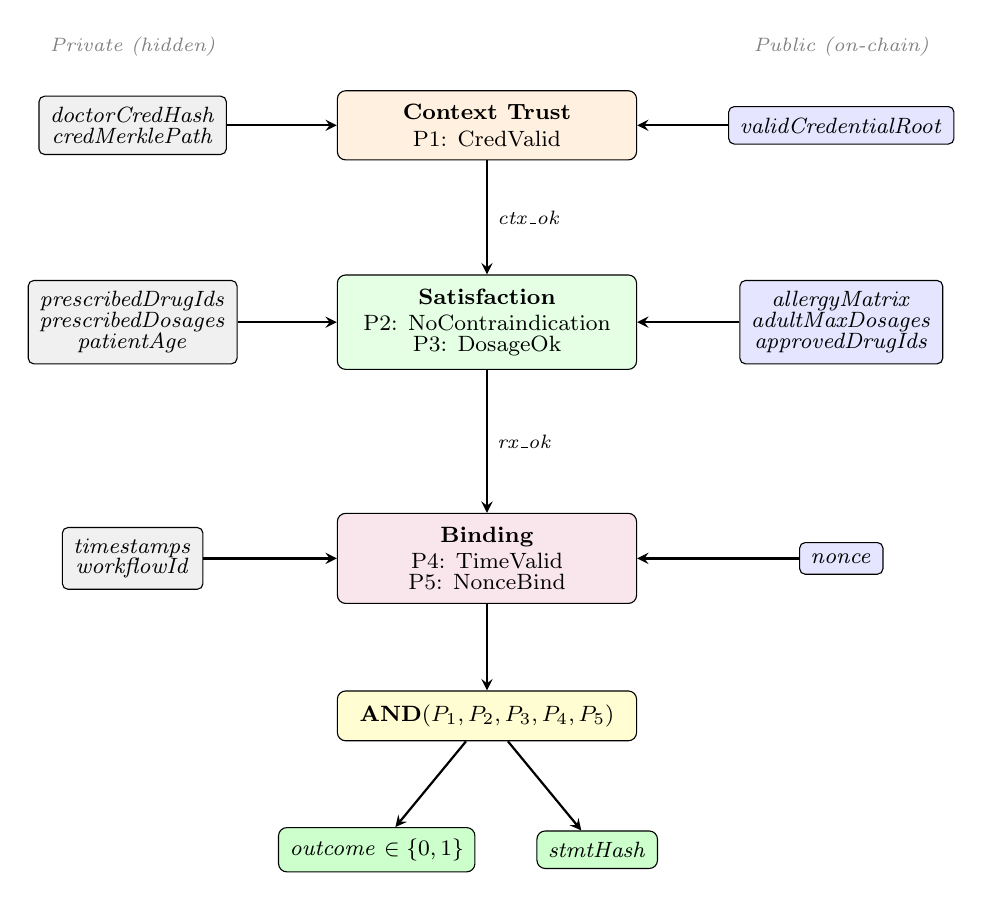
\begin{tikzpicture}[
  font=\footnotesize, >=stealth,
  priv/.style={draw, fill=gray!12, rounded corners=2pt,
               inner sep=4pt, align=center},
  pub/.style={draw, fill=blue!10, rounded corners=2pt,
               inner sep=4pt, align=center},
  blk/.style={draw, rounded corners=3pt, inner sep=5pt,
               align=center, minimum width=3.8cm},
  ctx/.style={blk, fill=orange!12},
  sat/.style={blk, fill=green!10},
  bnd/.style={blk, fill=purple!10},
  andblk/.style={blk, fill=yellow!18},
  outblk/.style={draw, fill=green!20, rounded corners=3pt,
               inner sep=4pt, align=center},
  arr/.style={->, thick}
]

\node[priv] (pr1) at (-4.5,  5.0)
  {\textit{doctorCredHash}\\[-2pt]\textit{credMerklePath}};
\node[priv] (pr2) at (-4.5,  2.5)
  {\textit{prescribedDrugIds}\\[-2pt]
   \textit{prescribedDosages}\\[-2pt]\textit{patientAge}};
\node[priv] (pr3) at (-4.5, -0.5)
  {\textit{timestamps}\\[-2pt]\textit{workflowId}};

\node[pub] (pu1) at (4.5, 5.0)
  {\textit{validCredentialRoot}};
\node[pub] (pu2) at (4.5, 2.5)
  {\textit{allergyMatrix}\\[-2pt]
   \textit{adultMaxDosages}\\[-2pt]\textit{approvedDrugIds}};
\node[pub] (pu3) at (4.5, -0.5)
  {\textit{nonce}};

\node[ctx] (ctx) at (0,  5.0)
  {\textbf{Context Trust}\\P1: CredValid};
\node[sat] (sat) at (0,  2.5)
  {\textbf{Satisfaction}\\
   P2: NoContraindication\\[-2pt]P3: DosageOk};
\node[bnd] (bnd) at (0, -0.5)
  {\textbf{Binding}\\
   P4: TimeValid\\[-2pt]P5: NonceBind};
\node[andblk] (andnode) at (0, -2.5)
  {$\mathbf{AND}(P_1,P_2,P_3,P_4,P_5)$};

\node[outblk] (oc) at (-1.4, -4.2)
  {\textit{outcome} $\in\{0,1\}$};
\node[outblk] (sh) at ( 1.4, -4.2)
  {\textit{stmtHash}};

\draw[arr] (pr1) -- (ctx);
\draw[arr] (pr2) -- (sat);
\draw[arr] (pr3) -- (bnd);
\draw[arr] (pu1) -- (ctx.east);
\draw[arr] (pu2) -- (sat.east);
\draw[arr] (pu3) -- (bnd.east);

\draw[arr] (ctx) -- node[right, font=\scriptsize]
  {$\mathit{ctx\_ok}$} (sat);
\draw[arr] (sat) -- node[right, font=\scriptsize]
  {$\mathit{rx\_ok}$} (bnd);
\draw[arr] (bnd)     -- (andnode);
\draw[arr] (andnode) -- (oc);
\draw[arr] (andnode) -- (sh);

\node[font=\scriptsize\itshape, gray] at (-4.5, 6.0)
  {Private (hidden)};
\node[font=\scriptsize\itshape, gray] at ( 4.5, 6.0)
  {Public (on-chain)};

\end{tikzpicture}%
}% end resizebox
\caption{Prescription validation circuit. Private patient data
and Merkle paths (left) are processed against
governance-approved public parameters (right).
Three sequential blocks enforce context trust, prescription
safety, and replay protection; the circuit emits
\textit{outcome} and \textit{stmtHash} as public outputs.}
\label{fig:circuit-flow}
\end{figure}

The semantic model~$M$, the governance-approved theory~$T$
are committed on the DKG through Merkle trees whose roots are
exposed as public inputs.
The first, $\mathit{root}_M$, follows the per-record leaf
pattern of verifiable-credential
systems~\cite{rosenberg2023zkcreds}:
each record $r \in M$, including physician credentials, is
encoded as a tuple of attributes and hashed into one leaf,
\begin{equation}
\mathit{leaf}(r) \;=\; H\bigl(
r_{\mathit{id}} \,\|\,
r_{\mathit{type}} \,\|\,
a_1 \,\|\, \dots \,\|\, a_k
\bigr),
\label{eq:leaf}
\end{equation}
where $r_{\mathit{id}}$ is the record identifier,
$r_{\mathit{type}}$ the record type, and $a_1,\dots,a_k$ the
record attributes.
Theory~$T$, including policy axioms
$\mathrm{Pol}(m,t,\mathit{op},\theta)$ and the subsumption
hierarchy, is committed as verified public circuit parameters
consumed by the corresponding sub-circuits.
Issuer signatures on credentials and source attestations are
verified off-circuit at registry inclusion.

Building on this commitment layer, the circuit decomposes
acceptance into two blocks whose outputs are multiplied into
a single acceptance flag $\mathit{outcome}\in\{0,1\}$:
the \emph{context-trust block} enforces
$\mathrm{ContextTrusted}(\Gamma,M)$
(Definition~\ref{def:context-trusted}), and the
\emph{satisfaction block} enforces
$M,\Gamma\models\mathrm{RxValid}(d,p,m,n)$
(Eq.~\ref{eq:rx-valid}).
The circuit is parameterised by~$N_{\max}$, the maximum
number of referenced records that can be carried in~$\Gamma$;
each reference slot supplies a Merkle membership proof
against $\mathit{root}_M$ together with the disclosed
attributes required by the satisfaction block.
Unused slots are padded with neutral values so that the
constraint structure remains fixed; padded slots satisfy all
per-reference checks tautologically.

The context-trust block consists of three sub-circuits.
The $\mathrm{CredValid}$ sub-circuit
($\mathit{credValid\_ok}$) verifies that $H(\mathit{cred})$ is
committed in $\mathit{root}_M$ through a Merkle membership
proof, without disclosing credential attributes.
The block output is
\begin{equation}
\mathit{ctx\_ok} = \mathit{credValid\_ok}.
\label{eq:ctx-flag}
\end{equation}
Per-record existence proofs are enforced at the system level
by the trusted prover infrastructure and deferred as an
in-circuit extension to future work.

The satisfaction block contains two sub-circuits.
The $\mathrm{NoContraindication}$ sub-circuit
($\mathit{no\_contra}$) checks whether any row of the
governance-approved public parameter $\mathit{allergyMatrix}$
has a $1$-entry for the prescribed medication~$m$.
Each entry $\mathit{allergyMatrix}[a][m]{=}1$ pre-encodes the
subsumption $s_a \sqsubseteq m$ (Eq.~\ref{eq:subsumption}),
computed off-chain by the governance process and committed as a
public circuit parameter; the circuit performs only the matrix lookup.
A positive match sets $\mathit{allergy\_contra}=1$;
otherwise $\mathit{no\_contra} = 1 - \mathit{allergy\_contra}$.
The $\mathrm{PolicySatisfied}$ sub-circuit
($\mathit{pol\_ok}$) enforces the policy axioms applicable
to~$m$: for each axiom
$\mathrm{Pol}(m,t,\mathit{op},\theta)$ (Eq.~\ref{eq:pol})
supplied as public circuit parameters, the circuit selects the
reference slot whose $\mathit{hasMetric}$ attribute matches~$t$
and enforces
$\mathit{hasValue}\;\mathit{op}\;\theta$ through a range-check
sub-circuit.
If no policy axioms apply to~$m$, $\mathit{pol\_ok}=1$
(vacuous satisfaction).
The prototype stratifies the dosage bound by patient age:
for patients under 11 years the circuit applies the private
$\mathit{childMaxDosages}$ thresholds; for adults it applies
the governance-approved public $\mathit{adultMaxDosages}$.
The block aggregates into
\begin{equation}
\mathit{rx\_ok}
=
\mathit{no\_contra}
\cdot
\mathit{pol\_ok}.
\label{eq:rx-flag}
\end{equation}

Combining the two block flags yields the final acceptance
flag:
\begin{equation}
\mathit{outcome}
=
\mathit{ctx\_ok}
\cdot
\mathit{rx\_ok},
\label{eq:outcome}
\end{equation}
which the circuit constrains to the public-input
$\mathit{outcome}$.
The circuit additionally recomputes $\mathit{stmt\_hash}$
(Eq.~\ref{eq:stmt-hash}) from the statement content and nonce
and constrains it to the corresponding public input, binding
the proof to a single prescription instance and governance
state.
All Boolean flags are constrained through $b(b-1)=0$.
An empirical instantiation of this circuit on the Metformin
case is reported in Section~\ref{ss:proof-gen}.

The witness and public-input split that supports this circuit
is structured as follows.
The private witness~$w$ groups all patient-specific evidence
and auxiliary values consumed by the circuit:
\begin{equation}
w =
\langle
w_{\mathrm{cred}},\;
w_{\mathrm{refs}},\;
w_{\mathrm{stmt}},\;
w_{\mathrm{ont}},\;
w_{\mathrm{aux}}
\rangle.
\label{eq:witness-struct}
\end{equation}
The \emph{credential witness}~$w_{\mathrm{cred}}$ carries the
credential $\mathit{cred}$ and its Merkle path against
$\mathit{root}_M$.
The \emph{reference witnesses}
$w_{\mathrm{refs}}^{1},\dots,w_{\mathrm{refs}}^{N_{\max}}$
each carry, for one reference slot~$r_i$, the record
identifier, type tag~$\tau_i$, and the disclosed attributes
required by the satisfaction block; unused slots are padded
with neutral values. Per-slot Merkle membership proofs against
$\mathit{root}_M$ are deferred to future work and enforced at
the system level by the trusted prover infrastructure.
The \emph{statement witness}~$w_{\mathrm{stmt}}$ carries the
prescription content $(\mathit{prescribedDrugIds}, \mathit{prescribedDosages})$
and is consumed jointly with $\mathit{doctorCredentialHash}$ and the
public nonce to compute $\mathit{stmtHash}$ in-circuit
(Eq.~\ref{eq:stmthash-instance}).
The \emph{ontology witness}~$w_{\mathrm{ont}}$ carries the
subsumption and policy-axiom values accessed from the
public theory parameters~$T$.
The \emph{auxiliary witness}~$w_{\mathrm{aux}}$ carries
intermediate Boolean flags, range-check auxiliaries, and
padding values.

The public input vector exposes only commitments and decision
metadata:
\begin{equation}
\begin{split}
\mathit{pub} = \langle\,
\underbrace{\mathit{outcome},\;\mathit{stmtHash}}_{\text{circuit outputs}},\;
\mathit{doctorCredentialHash},\; \\
\mathit{validCredentialRoot},\;
\mathit{nonce},\;
\mathit{approvedDrugIds},\; \\
\mathit{allergyMatrix},\;
\mathit{adultMaxDosages}
\,\rangle.
\end{split}
\label{eq:public-inputs}
\end{equation}
Here $\mathit{outcome}\in\{0,1\}$ is the acceptance decision
output by the circuit. The in-circuit commitment
\begin{equation}
\begin{split}
\mathit{stmtHash} = \mathrm{Poseidon}(&\mathit{dCH},\;\mathit{nonce},\\
&\mathit{prescribedDrugIds},\;\mathit{prescribedDosages})
\end{split}
\label{eq:stmthash-def}
\end{equation}
binds the proof to one prescription instance without disclosing
the prescription content on-chain, where $\mathit{dCH}$ abbreviates
$\mathit{doctorCredentialHash}$.
$\mathit{doctorCredentialHash}$ identifies the prescribing
doctor's credential leaf;
$\mathit{validCredentialRoot}$ pins the proof to the DKG-anchored
credential registry~($\mathit{root}_M$);
$\mathit{nonce}$ enforces per-workflow uniqueness; and
$\mathit{approvedDrugIds}$, $\mathit{allergyMatrix}$,
$\mathit{adultMaxDosages}$ pin the proof to the
governance-approved policy parameters~$T$.


Patient identifiers, prescribed drug identities, dosages,
clinical values, and credential attributes are confined
to~$w$ and never disclosed on chain; the verifier observes
only $\mathit{stmtHash}$ as a binding commitment to the
prescription content. The public input vector therefore
reveals only the acceptance decision, the prescription
commitment, and the governance-approved artifacts against
which the decision was verified.



\begin{proposition}[Compilation Soundness]
\label{prop:compile-soundness}
Let $C$ be the arithmetic circuit constructed above, encoding
$\mathrm{Accept}(M,\Gamma,\varphi^{+}_{Rx})$ for
$\varphi^{+}_{Rx}=\mathrm{RxValid}(d,p,m,n)$ over the
commitment scheme of Eq.~\ref{eq:leaf}.
If $C(w,x)=1$ for a witness~$w$ and a public input~$x$ whose
$\mathit{root}_M$ component equals the DKG-anchored
commitment to~$M$, and whose theory parameters equal the
governance-approved values of~$T$,
then
$\mathrm{Accept}(M,\Gamma,\varphi^{+}_{Rx})=\mathsf{true}$
under $M \models T$.
\end{proposition}

\begin{proof}[Proof sketch]
The acceptance predicate decomposes into
$\mathrm{ContextTrusted}(\Gamma,M)$ and
$M,\Gamma \models \mathrm{RxValid}(d,p,m,n)$
(Definitions~\ref{def:context-trusted}--\ref{def:acceptance}),
encoded respectively by the context-trust and satisfaction
blocks above.
Merkle membership against $\mathit{root}_M$ enforces
record existence and credential validity;
the public theory parameters enforce the ontology and policy
axioms of~$T$ consumed by the subsumption and policy-satisfaction sub-circuits;
range-check sub-circuits enforce the policy thresholds over
the disclosed values.
If $C(w,x)=1$, every sub-circuit flag evaluates to~$1$.
By collision resistance of~$H$ and the binding property of
Merkle commitments, each disclosed attribute is bound to a
leaf in $\mathit{root}_M$;
since the public input pins $\mathit{root}_M$ to the DKG-anchored
commitment to~$M$ and the theory parameters to the governance-approved~$T$,
the witnessed records are elements of~$M$, and the witnessed axioms
belong to~$T$.
Definitions~\ref{def:satisfaction}
and~\ref{def:acceptance} then yield
$\mathrm{Accept}(M,\Gamma,\varphi^{+}_{Rx})=\mathsf{true}$.
\end{proof}



\subsection{Proof Lifecycle and Governance Integration}
\label{sec:proof-lifecycle}

A proof is bound to three orthogonal artifacts.
The statement commitment $\mathit{stmt\_hash}$
(Eq.~\ref{eq:stmt-hash}) binds it to one ground statement
and one workflow invocation via the per-statement nonce.
The DKG-anchored commitment $\mathit{root}_M$ exposed
in $\mathit{pub}$ (Eq.~\ref{eq:public-inputs}) binds it to
the specific version of~$M$, and the public theory parameters
bind it to the specific version of~$T$ against which it was
generated.
The verification key~$\mathit{vk}$ binds it to the circuit
structure: once governance approves a revised circuit
(e.g., a new clause added to the satisfaction block), a new
$\mathit{vk}$ is published and proofs generated under the
previous circuit are no longer accepted.

Theory updates that change policy parameters require
the DAO to re-anchor the updated values on the DKG and
publish a new reference configuration; proofs generated
under prior parameter values will not match the on-chain
reference and fail verification. Updates that change the
circuit structure require a new trusted-setup ceremony
and a new~$\mathit{vk}$.


The same mechanism handles credential revocation: removing
a credential leaf from $\mathit{root}_M$ updates the
registry, and subsequent proofs invoking the revoked
credential fail the $\mathrm{CredValid}$ check
(Section~\ref{sec:rx-circuit}) without requiring a separate
revocation list.

At the on-chain verification layer, the verifier
(Section~\ref{sec:governance-layer}) performs the Groth16
pairing check automatically for every submitted proof and
appends the outcome together with $\mathit{stmt\_hash}$ to
the immutable acceptance log; any third party can audit the
decision through commitments alone, without access to
patient evidence.
The artifact $(\pi,\mathit{pub})$ is reusable: once verified
at issuance time, it can be presented to downstream
operational actors---e.g., a pharmacy at dispensing
time---which re-run the same verification against the
current DKG state, without re-evaluating semantic
conditions.

\subsection{Security and Privacy Analysis}
\label{sec:security-privacy-analysis}

We now establish that the construction satisfies the four
security goals declared in
Section~\ref{ss:threat-model}.

Correctness follows from zk-SNARK soundness.
If the on-chain verifier accepts a proof~$\pi$ with public
input~$x$, then by zk-SNARK soundness all circuit constraints
hold for the witness~$w$ supplied by the prover, and by
Proposition~\ref{prop:compile-soundness}
$\mathrm{Accept}(M,\Gamma,\varphi^{+})=\mathsf{true}$ under
$M \models T$.
A dishonest prover, including one colluding with a malicious
semantic interpreter, therefore cannot obtain acceptance for
a statement that fails the encoded semantic conditions
without breaking Groth16 soundness or the collision
resistance of~$H$.
A governance-level adversary controlling fewer than the
required DAO votes cannot modify~$T$, the registries,
or~$\mathit{vk}$ to coerce acceptance; unauthorised
modifications produce DKG commitments that fail to match the
proof's public input.

Privacy holds because all patient-specific evidence is
confined to the private witness~$w$
(Eq.~\ref{eq:witness-struct}).
Under the zero-knowledge property of Groth16, $\pi$ reveals
no information about~$w$ beyond what is already entailed by
$\mathit{pub}$ (Eq.~\ref{eq:public-inputs}).
The governance layer and any external observer therefore
learn only the acceptance outcome together with commitments
to the governance-approved artifacts; patient identifiers,
medication identities, clinical values, credential
attributes, and the specific subsumption and policy paths
traversed in~$T$ remain undisclosed.

Binding holds because each proof is cryptographically pinned to
(i)~the specific prescription instance and workflow invocation
through $\mathit{stmtHash}$,
(ii)~the governance state through $\mathit{validCredentialRoot}$
and the public theory parameters, and
(iii)~the circuit structure through~$\mathit{vk}$
(Section~\ref{sec:proof-lifecycle}).
A proof generated under any other instance, governance state,
or circuit version fails verification.
Replay across workflows is prevented by the per-workflow
nonce included in $\mathit{stmtHash}$.

Governance verifiability is achieved because verification
requires only $(\pi, \mathit{pub})$ together
with the current DKG-anchored commitments; no privileged
access to~$M$, $T$, or patient evidence is required.
Any third party with read access to the on-chain log and the
DKG can therefore independently re-verify any past
acceptance decision, and the immutable log
(Section~\ref{sec:governance-layer}) provides a permanent
audit trail keyed by $\mathit{stmt\_hash}$.

Several limitations and scope boundaries apply.
(i)~Groth16 requires a per-circuit trusted setup; if all
contributors to the ceremony collude, soundness can be
weakened. This risk is mitigated by the multi-contributor
ceremony of Section~\ref{ss:ceremony}.
(ii)~Proposition~\ref{prop:compile-soundness} closes the gap
between Definitions~\ref{def:context-trusted}--\ref{def:acceptance}
and the arithmetic circuit; the gap between the circuit
specification and its deployed Circom implementation must be
closed by circuit auditing.
(iii)~Public metadata---in particular $t_{\mathrm{req}}$ and
the frequency of acceptance events---can support limited
traffic-analysis inference even though individual proofs
reveal no PHI; the per-statement nonce prevents cross-workflow
linkage of acceptance events.
(iv)~The protocol guarantees compliance with the
governance-approved theory~$T$ but does not validate~$T$
itself; clinical correctness of the encoded policy axioms
remains the responsibility of the governance authority that
approves them.


\subsection{Complexity Analysis}
\label{sec:complexity-analysis}

We characterise the circuit complexity analytically;
empirical measurements that instantiate the constants below
are reported in Section~\ref{ss:performance}.

The constraint count is dominated by three sub-circuit
families: credential verification ($n_{\mathrm{cred}}$),
Merkle membership proofs against $\mathit{root}_M$ ($n_{\mathrm{Merkle}}$ per
proof), and range checks for policy
satisfaction ($n_{\mathrm{range}}$ per axiom).
Let $|\mathrm{PolicyAxioms}(m,T)|$ denote the number of
policy axioms applicable to medication~$m$, with at most one
subsumption check per reference slot.
The total constraint count is approximately
\begin{equation}
\begin{split}
n_{\mathrm{total}} \;\approx\;\;
&n_{\mathrm{cred}}
+ N_{\max} \cdot n_{\mathrm{Merkle}} \\
+ |\mathrm{PolicyAxioms}(m,T)| \cdot n_{\mathrm{range}},
\end{split}
\label{eq:complexity}
\end{equation}
where the $N_{\max}$ factor reflects one Merkle path against
$\mathit{root}_M$ per reference slot.

The complexity is therefore linear in~$N_{\max}$ and in the
number of applicable policy axioms, while $n_{\mathrm{cred}}$
and the per-proof constants depend only on the depth of the
Merkle trees and on the choice of hash function.
Doubling~$N_{\max}$ doubles only the per-reference terms;
the credential and policy components are unchanged.

The choice of zk-SNARK back-end determines proof size, prover
cost, and on-chain verification cost; the concrete
instantiation used in this work is reported in
Section~\ref{ss:performance}.
For the practical SNARK families considered, proofs remain
succinct and on-chain verification cost depends primarily on
the size of the public input vector~$\mathit{pub}$
(Eq.~\ref{eq:public-inputs}) rather than on the circuit size,
so computational effort is concentrated off-chain at proving
time.


\section{Evaluation}
\label{s:eval}

This section reports the implementation and empirical evaluation of the
\textsc{PrescriptionValidation} zero-knowledge circuit described in
Section~\ref{s:rq3}.
The evaluation covers three aspects: the reproducible trusted-setup ceremony that
generated the proving and verification keys, the proof-generation and verification
run for the Metformin running case, and a scenario-based validation suite that
exercises every security property of the circuit.

\subsection{DKG Knowledge Graphs}
\label{ss:dkg-knowledge-graphs}

This subsection presents the concrete RDF representation of the three
DKG artifacts that ground the prescription validation circuit:
medical rules and policies, patient clinical data,
and the prescription request context. Each artifact
is serialized in Turtle syntax and corresponds to one input class
consumed by the circuit (Section~\ref{sec:rx-circuit}). The full
ontology together with all instances is publicly available
at\footnote{\url{https://github.com/medalex/zkp-prescription-ontology}}.
The ontology imports the MFSSIA ontology via \texttt{owl:imports}
and was validated for consistency using the Pellet OWL-DL
reasoner~\cite{pellet}.

\paragraph{Medical Rules and Policies (Theory $T$)}
Listing~\ref{lst:rules} encodes a fragment of the
governance-approved theory~$T$: an ontological subsumption between
medication classes and a clinical policy axiom for Metformin. These
artifacts are consumed by the NoContraindication sub-circuit
(via lookup in the pre-computed $\mathit{allergyMatrix}$) and by the PolicySatisfied
sub-circuit (via range-check constraints over the policy threshold).

\begin{lstlisting}[caption={Medical Rules and Policies},label={lst:rules},language=turtle,basicstyle=\ttfamily\footnotesize]
rx:Penicillin a rx:MedicationClass ;
    rx:subsumes rx:BetaLactam .

rx:PolicyMetforminEGFR a rx:ClinicalPolicy ;
    rx:appliesToMedication rx:Metformin ;
    rx:clinicalCondition "eGFR" ;
    rx:comparisonOperator ">=" ;
    rx:threshold 30 .
\end{lstlisting}

\paragraph{Patient Clinical Data (Records in $M$)}
Listing~\ref{lst:patient} shows the labeled records for the running
case patient: a Penicillin allergy and a recent eGFR measurement.
These records reside off-chain and enter the circuit only as private
witness inputs (Section~\ref{sec:rx-circuit}); their existence
in~$M$ is attested through Merkle membership proofs against
$\mathit{root}_M$.

\begin{lstlisting}[caption={Patient Clinical Data},label={lst:patient},language=turtle,basicstyle=\ttfamily\footnotesize]
rx:AllergyPat1Penicillin a rx:Allergy ;
    rx:allergicToSubstance rx:Penicillin ;
    rx:snomedCode "416098002" .

rx:LabEGFRpat1 a rx:LabResult ;
    rx:conditionType "eGFR" ;
    rx:clinicalValue "45"^^xsd:decimal ;
    rx:measuredBy rx:DiagLab1 .
\end{lstlisting}

\paragraph{Prescription Request Context ($\Gamma$)}
Listing~\ref{lst:context} captures the evaluation context for a
specific prescription request: the data source, request timestamp,
and a coarse time anchor used as a public input.

\begin{lstlisting}[caption={Prescription Request Context},label={lst:context},language=turtle,basicstyle=\ttfamily\footnotesize]
rx:EvalCtx_Prescription1 a rx:EvaluationContext ;
    rx:hasDataSource rx:DiagLab1 ;
    rx:contextTimestamp "2026-04-08T10:00:00"^^xsd:dateTime ;
    rx:tsAnchor 90 .
\end{lstlisting}

Together these four artifacts populate the DKG with all
governance-approved knowledge required for circuit evaluation. The
prover assembles the private witness by retrieving the relevant
records from~$M$, the applicable axioms from~$T$, and constructs
Merkle authentication paths against the DKG-anchored commitments.
No clinical attribute leaves the prover's domain; the governance
layer observes only the proof~$\pi$ and the public input vector
of Eq.~\ref{eq:public-inputs}.

% ─────────────────────────────────────────────────────────────────────────────
\subsection{Trusted Setup Ceremony}
\label{ss:ceremony}
% ─────────────────────────────────────────────────────────────────────────────



% ─────────────────────────────────────────────────────────────────────────────
\subsection{Proof Generation and Verification}
\label{ss:proof-gen}
% ─────────────────────────────────────────────────────────────────────────────

The canonical proof instance uses the following concrete values.
Private inputs are:
$\mathit{prescribedDrugIds} = [101, 104]$,
$\mathit{prescribedDosages} = [8, 2]$,
$\mathit{patientAge} = 12$,
$\mathit{prescriptionTimestamp} = 1000$,
$\mathit{validFor} = 50$,
$\mathit{currentTimestamp} = 1030$,
$\mathit{workflowId} = 77$,
$\mathit{credentialSiblings} = [666, 8729\ldots, 2627\ldots]$,
$\mathit{credentialPathBits} = [0, 0, 1]$,
$\mathit{childMaxDosages} = [10, 5, 8, 2]$.

\noindent
The statement commitment is computed in-circuit as
\begin{equation}
\mathit{stmtHash}
  = \mathrm{Poseidon}(\mathit{dCH},\,\mathit{nonce},\,101,\,104,\,8,\,2)
  = \mathit{XXX}
\label{eq:stmthash-instance}
\end{equation}
where $\mathit{dCH} = \mathit{doctorCredentialHash} = 555$ and
$\mathit{nonce} = \mathrm{Poseidon}(77) = \mathit{XXX}$.

\noindent
The public input vector submitted to the verifier is:
\begin{align*}
\vec{x} = [&\,\underbrace{\mathit{XXX}}_{\mathit{stmtHash}},\;
             \underbrace{1}_{\mathit{outcome}},\;
             \underbrace{555}_{\mathit{dCH}},\\
           &\underbrace{12637\ldots}_{\mathit{validCredentialRoot}},\;
            \underbrace{\mathit{XXX}}_{\mathit{nonce}},\\
           &\underbrace{[101,102,103,104]}_{\mathit{approvedDrugIds}},\;
            \underbrace{[20,10,16,4]}_{\mathit{adultMaxDosages}},\\
           &\underbrace{[[0,0,1,0],\ldots]}_{\mathit{allergyMatrix}}\,].
\end{align*}

The witness was generated by the compiled WebAssembly module
(\texttt{prescription.wasm}) and the proof $\pi = (\pi_a, \pi_b, \pi_c)$
was computed with \texttt{snarkjs groth16 prove}.
The Groth16 verifier executed the pairing check
$e(\pi_a, \pi_b) = e(\mathsf{vk\_alpha\_1}, \mathsf{vk\_beta\_2}) \cdot
e(\mathsf{vk\_alphabeta\_12}) \cdot
e(\pi_c, \mathsf{vk\_delta\_2})$ and returned \textbf{Proof valid: true}.
The proof occupies 192~bytes (three BN128 elliptic-curve points).

% ─────────────────────────────────────────────────────────────────────────────
\subsection{Scenario-Based Validation}
\label{ss:scenarios}
% ─────────────────────────────────────────────────────────────────────────────

Twelve scenarios were designed to cover every constraint and security
property of the circuit, organized into five categories: completeness
tests, context-trust soundness tests (one per predicate), satisfaction soundness tests
(one per clause of Definition~\ref{def:satisfaction}), binding and
replay tests, and scalability tests.
Table~\ref{tab:scenarios} summarizes the results; all twelve passed.

\begin{table}[h]
\centering
\caption{Scenario-based validation results (12/12 passed).}
\label{tab:scenarios}
\footnotesize
\renewcommand{\arraystretch}{1.1}
\begin{tabular}{c l c c l}
\toprule
\textbf{ID} & \textbf{Scenario} &
  \textbf{Proof} & \textbf{Verify} & \textbf{Result} \\
\midrule
\multicolumn{5}{l}{\textit{Completeness (positive tests)}} \\
S1    & Valid baseline (Metformin, $N_{\max}{=}5$)    & \checkmark & \checkmark & Pass \\
S5a   & Honest reject (contraindication)              & \checkmark & \checkmark & Pass \\
S10   & Honest reject (policy violation)              & \checkmark & \checkmark & Pass \\
S13   & Minimal refs (1 of 5 populated)               & \checkmark & \checkmark & Pass \\
\midrule
\multicolumn{5}{l}{\textit{Context-trust soundness (Definition~\ref{def:context-trusted})}} \\
S2    & $\mathrm{CredValid}$ failure (cred not in registry) & $\times$ & $\times$ & Pass  \\
\midrule
\multicolumn{5}{l}{\textit{Satisfaction soundness (Definition~\ref{def:satisfaction})}} \\
S5b   & Forged accept (contraindication)              & $\times$   & $\times$   & Pass \\
S11   & Forged accept (policy violation)              & $\times$   & $\times$   & Pass \\
\midrule
\multicolumn{5}{l}{\textit{Binding and replay}} \\
S6    & Replay / tampered public signals              & reuse      & $\times$   & Pass \\
S7    & Wrong verification key                        & reuse      & $\times$   & Pass \\
\midrule
\multicolumn{5}{l}{\textit{Scalability}} \\
S12   & Scalability test ($N_{\max}{=}10$, 10 refs)   & \checkmark & \checkmark & Pass \\
\bottomrule
\end{tabular}
\end{table}

\paragraph{S1 --- Valid Baseline.}
The Metformin running case of Section~\ref{ss:rc}
with $N_{\max} = 5$. The evaluation context
$\Gamma_H = \langle \mathit{cred}_{\mathit{doc}_1}, \{a_2, l_3\},
20561 \rangle$ populates two reference slots and pads the
remaining three. The $\mathrm{ContextTrusted}$ predicate holds,
both $\mathrm{RxValid}$ clauses hold, and the circuit evaluates
$\mathit{ctx\_ok} = 1$, $\mathit{rx\_ok} = 1$, 
$\mathit{outcome} = 1$, matching the declared public input.
Proof generation and on-chain verification both succeed.

\paragraph{S2 --- CredValid Failure.}
The physician's credential has been removed from the
governance-approved registry: the issuing authority has
published an updated $\mathit{root}_M$ that no longer
contains the credential leaf. The prover attempts to supply
a Merkle authentication path for $H(\mathit{cred})$ against
the updated $\mathit{root}_M$, but no valid path exists.
$\mathit{credValid\_ok} = 0$, forcing $\mathit{ctx\_ok} = 0$,
and witness generation aborts. This confirms that revocation
is enforced through $\mathit{root}_M$ updates without
requiring a separate on-chain revocation list.

\paragraph{S5a --- Honest Reject: Contraindication.}
The allergy record $a_2$ carries
$\mathit{hasSubstance} = \mathrm{Penicillin}$, and the prescribed
medication belongs to the $\beta$-lactam class
($\mathrm{Penicillin} \sqsubseteq \beta\text{-lactam}$). The
subsumption witness $m \sqsubseteq s$ is produced, setting
$\mathit{allergy\_contra} = 1$ and
$\mathit{no\_contra} = 0$. Consequently $\mathit{rx\_ok} = 0$ and
$\mathit{outcome} = 0$. The prover honestly declares
$\mathit{outcome} = 0$; the final equality constraint passes and a
valid \emph{rejection proof} is produced. This proof is auditable
on-chain: any verifier can confirm the prescription was correctly
refused without learning the patient's allergy substance.

\paragraph{S5b --- Forged Accept: Contraindication.}
Same evidence as S5a, but the prover claims
$\mathit{outcome} = 1$. The circuit computes
$\mathit{computedOutcome} = 0 \neq 1$; the final equality constraint
fails. Together with S5a, this pair establishes
\emph{outcome integrity}: the prover can publish only the outcome
that the circuit actually computes, never a different one.

\paragraph{S10 --- Honest Reject: Policy Violation.}
The laboratory result carries $\mathit{hasValue} = 25$, violating
the policy axiom
$\mathrm{Pol}(\mathrm{Metformin}, \mathrm{eGFR}, {\geq}, 30)$. The
range-check sub-circuit sets $\mathit{pol\_ok} = 0$,
$\mathit{rx\_ok} = 0$, $\mathit{outcome} = 0$. The prover honestly
declares rejection; a valid \emph{rejection proof} is produced.
Analogous to S5a, this demonstrates that policy-based rejections are
auditable without revealing the underlying clinical value (only that
the threshold was not met).

\paragraph{S11 --- Forged Accept: Policy Violation.}
Same evidence as S10 ($\mathit{hasValue} = 25$), but the prover
claims $\mathit{outcome} = 1$. The range-check sub-circuit evaluates
$25 \geq 30$ to false, so $\mathit{pol\_ok} = 0$ and
$\mathit{computedOutcome} = 0 \neq 1$. The final equality constraint
fails. This extends outcome integrity to the policy clause: clinical
threshold violations cannot be hidden by a dishonest prover.

\paragraph{S6 --- Replay / Substitution Attack.}
The valid proof $\pi$ from S1 is reused without modification, but
the public input $\mathit{publicSignals}[\mathit{outcome}]$ is
flipped from $1$ to $0$. The Groth16 pairing equations are binding
over the exact public-input vector; any modification invalidates the
proof, so
$\mathrm{Verify}(\pi_{\mathrm{S1}}, \vec{x}\,{}') = \mathbf{false}$.

\paragraph{S7 --- Wrong Verification Key.}
The valid proof and public signals from S1 are submitted to a
verifier whose $\mathit{IC}[0][0]$ coefficient has been corrupted
(simulating a governance key update after a circuit revision). The
pairing check fails because $\mathit{vk}$ is bound to the exact
circuit. In production, governance deploys a new
\texttt{PrescriptionVerifier.sol} after each circuit revision;
proofs generated under the previous key are not accepted.

\paragraph{S13 --- Minimal Refs with Padding.}
Only one reference slot is populated (a laboratory result $l_3$ 
matching the single policy axiom for the prescribed medication), 
and the remaining four slots are padded with
canonical zero-attribute values. Padded slots satisfy all three
per-reference sub-circuits tautologically, contributing $1$ to
$\mathit{ctx\_ok}$ (Eq.~\ref{eq:ctx-flag}). The satisfaction block
holds: $\mathrm{NoContraindication}$ holds vacuously (no
allergy records present), and $\mathrm{PolicySatisfied}$ is 
satisfied by the laboratory value against the single applicable 
policy axiom. $\mathit{outcome} = 1$ is produced. This
confirms that padded slots preserve circuit semantics without
introducing spurious rejections, and documents the constraint cost
floor when fewer references are needed.

\paragraph{S12 --- Scalability Test ($N_{\max} = 10$).}
The circuit is recompiled with $N_{\max} = 10$, and ten reference
slots are populated (four allergy records and six laboratory 
results for different policy axioms). All three
$\mathrm{ContextTrusted}$ predicates and both
$\mathrm{RxValid}$ clauses hold. Proof generation and verification
both succeed. The constraint count approximately doubles the
per-reference term of Eq.~\ref{eq:complexity} compared to S1; the
verification cost on-chain remains constant due to the succinctness
of Groth16.

\medskip
\noindent
Table~\ref{tab:coverage} maps each circuit constraint class to the
scenarios that exercise it.

\begin{table}[h]
\centering
\caption{Constraint coverage by scenario.}
\label{tab:coverage}
\footnotesize
\renewcommand{\arraystretch}{1.1}
\begin{tabular}{l p{3.8cm}}
\toprule
\textbf{Constraint class} & \textbf{Covered by} \\
\midrule
Statement binding $\mathit{stmt\_hash}$    & S1, S5a, S10 (pos.); \\
$\mathrm{CredValid}$ sub-circuit            & S2 (neg.) \\
$\mathrm{NoContraindication}$ sub-circuit   & S5a, S5b \\
$\mathrm{PolicySatisfied}$ sub-circuit      & S10, S11 \\
Outcome composition equality                & S5b, S11 (neg.); S1, S5a, S10 (pos.) \\
Groth16 / public-input binding              & S6 \\
Groth16 / verification-key binding          & S7 \\
Padding slot tautology                      & S13 \\
Scalability ($N_{\max} = 10$)               & S12 \\
\bottomrule
\end{tabular}
\end{table}

\medskip
\noindent
The scenarios confirm six security properties that, together,
realise the four goals declared in
Section~\ref{ss:threat-model}:
\emph{completeness} (S1, S5a, S10, S13, S12),
\emph{soundness} (S2, S5b, S11),
\emph{zero-knowledge} (architectural guarantee of the proof
system, inherited by all scenarios),
\emph{outcome integrity} (S5a+S5b, S10+S11),
\emph{replay resistance} (S6), and
\emph{key binding} (S7).

% ─────────────────────────────────────────────────────────────────────────────
\subsection{Performance Evaluation}
\label{ss:performance}
% ─────────────────────────────────────────────────────────────────────────────

While Section~\ref{ss:scenarios} establishes functional correctness
through scenario-based validation, this subsection quantifies the
computational cost of proof generation and verification as a
function of the number of reference slots populated in~$\Gamma$.
All measurements were obtained on a commodity laptop
(specify: CPU, RAM, OS) using \texttt{snarkjs}~0.7.6 and
\texttt{circom}~2.0. Reported times are means over ten runs.

\paragraph{Constraint scaling within the main circuit ($N_{\max} = 5$).}
Table~\ref{tab:perf-main} reports the total constraint count,
proof-generation time, and on-chain verification cost as the number
of populated reference slots varies from one to five, with the
remaining slots padded. Padding contributes a small fixed overhead
per unused slot (tautological satisfaction of the per-reference
sub-circuits), while the per-reference cost grows approximately
linearly with the number of populated slots, as predicted by
Eq.~\ref{eq:complexity}.

\begin{table}[h]
\centering
\caption{Performance of the main circuit ($N_{\max} = 5$) as a
function of populated reference slots.}
\label{tab:perf-main}
\footnotesize
\renewcommand{\arraystretch}{1.1}
\begin{tabular}{c c c c c}
\toprule
\textbf{Refs} & \textbf{Constraints} & \textbf{Wires} &
\textbf{Prove (ms)} & \textbf{Verify (ms)} \\
\midrule
1 & XXX & XXX & XX.X & X.X \\
2 & XXX & XXX & XX.X & X.X \\
3 & XXX & XXX & XX.X & X.X \\
4 & XXX & XXX & XX.X & X.X \\
5 & XXX & XXX & XX.X & X.X \\
\bottomrule
\end{tabular}
\end{table}

Proof size is constant at 192~bytes (three BN128 elliptic-curve
points) and independent of the number of reference slots, as
guaranteed by Groth16~\cite{groth2016}.

\paragraph{Scalability beyond the main circuit ($N_{\max} = 10$).}
To demonstrate that the circuit design scales beyond the default
deployment, we recompiled the circuit with $N_{\max} = 10$ and
measured its performance at the upper bound. Table~\ref{tab:perf-scale}
compares the two configurations at their maximum populated load.

\begin{table}[h]
\centering
\caption{Comparison of main ($N_{\max} = 5$) and scalability
($N_{\max} = 10$) configurations at maximum load.}
\label{tab:perf-scale}
\footnotesize
\renewcommand{\arraystretch}{1.1}
\begin{tabular}{l c c}
\toprule
\textbf{Metric} & $\mathbf{N_{\max} = 5}$ & $\mathbf{N_{\max} = 10}$ \\
\midrule
Total constraints        & XXX  & XXX  \\
Wires                    & XXX  & XXX  \\
Trusted-setup time (s)   & XX.X & XX.X \\
Proving key size (MB)    & XX.X & XX.X \\
Proof generation (ms)    & XX.X & XX.X \\
On-chain verification (ms) & X.X & X.X \\
Proof size (bytes)       & 192  & 192  \\
\bottomrule
\end{tabular}
\end{table}

The per-reference term of Eq.~\ref{eq:complexity} approximately
doubles between the two configurations, while the credential and
satisfaction components remain unchanged. On-chain verification cost
is identical across configurations and independent of circuit
complexity, as it requires a fixed number of elliptic-curve pairing
operations determined only by the number of public inputs. Proof
size is also identical, confirming the succinctness property of
Groth16.

\paragraph{Practical feasibility.}
For the main $N_{\max} = 5$ configuration, proof generation completes
within XX~ms on commodity hardware, comfortably below the
interactive latency requirements of clinical prescription workflows
(seconds). On-chain verification costs approximately XX~gas units on
Ethereum, enabling cost-predictable governance-layer integration.
The $N_{\max} = 10$ configuration increases proof-generation time by
approximately $\mathit{XX}\%$ while preserving the same verification
characteristics, demonstrating that the circuit design accommodates
complex prescription workflows (multiple allergies, several
laboratory criteria) without architectural changes.

\paragraph{Comparison with related approaches.}
Compared to Multi-Party Computation, our approach avoids synchronous
interaction between parties: proof generation is performed by a
single prover off-chain, and verification is non-interactive.
Compared to Homomorphic Encryption, it provides verifiable
correctness of semantic decisions rather than opaque ciphertext
arithmetic. Compared to zk-SNARK systems that encode only numerical
constraints on data values, our circuit encodes first-order logical
conditions over labeled facts in~$M$ (context trust, satisfaction
clauses, statement binding), extending Merkle-based commitment
patterns from data-level membership proofs to governance-level
semantic consensus.

\section{Discussions}
\label{s:discussions}

\section{Conclusion}
\label{s:conclusion}


\appendices
\section{Consolidated Notation Reference}
\label{app:notation}

Table~\ref{tab:notation} consolidates the notation used throughout this paper.

\begin{table*}[!ht]
\centering
\caption{Consolidated Notation Reference}
\label{tab:notation}
\footnotesize
\renewcommand{\arraystretch}{0.95}
\begin{tabular}{p{4.5cm} p{1.4cm} p{10.5cm}}
\toprule
\textbf{Symbol} & \textbf{Reference} & \textbf{Description} \\
\midrule

\multicolumn{3}{l}{\textit{Semantic Model and Domain}} \\
$M = \langle D, I \rangle$ & Eq.~\ref{eq:model} & Shared semantic model: domain $D$ and interpretation function $I$ \\
$D = D_P \uplus D_S \uplus D_M \uplus D_D$ & Def.~2 & Typed domain: patients, substances, medications, prescribers (pairwise disjoint) \\
$T = \{\alpha_1, \ldots, \alpha_n\}$ & Eq.~\ref{eq:theory} & Governance-approved theory: structural axioms, alignment bridges, clinical policy axioms \\
$M \models T$ & \S~II-C & Model $M$ satisfies all axioms in theory $T$ (admissibility precondition) \\
$M, \Gamma \models \varphi$ & Def.~2 & Extended Tarski satisfaction (partial relation: defined only when $\mathrm{ContextTrusted}(\Gamma, M)$) \\
$\varphi$;\; $\varphi^{+}$ & \S~III, IV-B & Statement schema; ground instantiation with concrete identifiers \\
$p \in D_P$;\; $s \in D_S$;\; $m \in D_M$;\; $d \in D_D$ & --- & Patient; substance/drug class; medication; prescriber \\
\midrule

\multicolumn{3}{l}{\textit{Labeled Facts in $M$ (RDF-style entity-attribute structure)}} \\
$I(\mathit{isAllergy})$, $I(\mathit{isLabResult})$ & \S~II-C & Type-membership relations identifying labeled record entities in $M$ \\
$I(\mathit{hasPatient})$, $I(\mathit{hasSubstance})$, $I(\mathit{hasMetric})$, $I(\mathit{hasValue})$ & \S~II-C & Attribute relations linking record entities to clinical content \\
$I(\mathit{hasPatientAttr})$ & Eq.~\ref{eq:attr-value} & Ternary relation linking patient to attribute name and value (age, weight, pregnancy status) \\
$I(\mathit{hasSource})$ & \S~II-C & Provenance attribute attached to each labeled record \\
\midrule

\multicolumn{3}{l}{\textit{Evaluation Context and Trust Predicates}} \\
$\Gamma = \langle \mathit{cred}, \mathit{refs}, t_{\mathit{req}} \rangle$ & Eq.~\ref{eq:ctx} & Evaluation context: credential, references to records in $M$, request timestamp \\
$\mathrm{CredValid}(\mathit{cred})$ & Def.~1 & Credential is included in the governance-approved credential registry committed in $\mathit{root}_M$ \\
$\mathrm{ContextTrusted}(\Gamma, M)$ & Def.~1 & Conjunction of all three trust predicates \\
$\mathrm{Accept}(M, \Gamma, \varphi)$ & Def.~3 & Governance acceptance: $\mathrm{ContextTrusted}(\Gamma, M) \wedge M, \Gamma \models \varphi$ \\
\midrule

\multicolumn{3}{l}{\textit{Clinical Predicates}} \\
$\mathrm{Allergy}(p, s)$ & Def.~2 & Labeled allergy record links patient $p$ to substance $s$ \\
$\mathrm{Contraindication}(p, m)$ & Def.~2 & Medication $m$ contraindicated for $p$ (via allergy + subsumption) \\
$\mathrm{PolicySatisfied}(p, m, n)$ & Def.~2 & All policy axioms for $m$ satisfied by $p$'s evidence (lab results, patient attributes) and prescribed dose $n$ \\
$\mathrm{RxValid}(d, p, m, n)$ & Def.~2 & Prescription validity: $\neg \mathrm{Contraindication} \wedge \mathrm{PolicySatisfied}$ \\
$\mathrm{Pol}(m, t, \mathit{op}, \theta)$ & Eq.~\ref{eq:pol} & Clinical policy axiom in $T$: medication $m$ subject to $t\;\mathit{op}\;\theta$ \\
$\mathrm{PolicyAxioms}(m, T)$ & Def.~2 & Set of policy triples $(t, \mathit{op}, \theta)$ in $T$ applicable to $m$ \\
$\sqsubseteq$ & Eq.~\ref{eq:subsumption} & Subsumption relation in the ontology (governance-approved hierarchy in $T$) \\
\midrule

\multicolumn{3}{l}{\textit{Cryptographic and Circuit Notation}} \\
$\pi$;\; $\mathit{vk}, \mathit{pk}$ & \S~V-B & Zero-knowledge proof; verification and proving keys \\
$w = \langle w_{\mathrm{cred}}, w_{\mathrm{refs}}, w_{\mathrm{stmt}}, w_{\mathrm{ont}}, w_{\mathrm{aux}} \rangle$ & Eq.~\ref{eq:witness-struct} & Private witness: credential, references, statement, ontology, auxiliary \\

$\mathit{pub} = \langle \mathit{outcome}, \mathit{stmtHash}, \mathit{doctorCredentialHash},$\newline $\mathit{validCredentialRoot}, \mathit{nonce}, \mathit{approvedDrugIds}, \mathit{allergyMatrix}, \mathit{adultMaxDosages} \rangle$ & Eq.~\ref{eq:public-inputs} & Public input vector for on-chain verification \\

$\mathit{stmtHash} = \mathrm{Poseidon}(\mathit{dCH},\,\mathit{nonce},\,\mathit{prescribedDrugIds},\,\mathit{prescribedDosages})$ & Eq.~\ref{eq:stmthash-instance} & In-circuit commitment binding prescription content and nonce \\

$\mathit{outcome} \in \{0, 1\}$ & \S~V-C & Accept (1) or reject (0) decision produced by the circuit \\
$C(w, x)$ & \S~V-B & Arithmetic circuit: outputs 1 iff semantic constraints hold \\
$\mathbb{F}$;\; $\mathrm{id}(\cdot)$;\; $H(\cdot)$ & \S~V-B & Finite field; identifier encoding; hash function \\
\bottomrule
\end{tabular}
\end{table*}


\section{Ontology Realization Tables}
\label{app:ontology-tables}

Tables~\ref{tab:ontology-classes} and~\ref{tab:ontology-dataprops}
detail the OWL~2 realization of the prescription extension introduced
in Section~\ref{ss:semantic}.

% TABLE Ia — OWL classes
\begin{table*}[tb]
\centering
\caption{OWL Classes of the Prescription Extension: DL Expressions and Formal Logical Representations}
\label{tab:ontology-classes}
\small
\begin{tabular}{p{2.0cm} p{2.0cm} p{3.6cm} p{5.8cm}}
\toprule
\textbf{Formal predicate} & \textbf{OWL class} & \textbf{DL expression} & \textbf{Formal logical representation} \\
\midrule

$\mathrm{RxValid}(d,p,m,n)$
  & \texttt{rx:Pre\-scrip\-tion}
  & \texttt{SubClassOf mfssia:Asset} \newline
    \texttt{prescribedBy exactly 1} \newline
    \texttt{~~rx:Physician} \newline
    \texttt{prescribes exactly 1} \newline
    \texttt{~~rx:Medication} \newline
    \texttt{prescribedFor exactly 1} \newline
    \texttt{~~rx:Patient}
  & $\forall x\;(x \in \mathtt{rx{:}Prescription} \;\to$
    $\;x \in \mathtt{mfssia{:}Asset}$
    $\;\wedge\; \exists!\,d\;(\mathtt{prescribedBy}(x,d) \wedge d \in D_D)$
    $\;\wedge\; \exists!\,m\;(\mathtt{prescribes}(x,m) \wedge m \in D_M)$
    $\;\wedge\; \exists!\,p\;(\mathtt{prescribedFor}(x,p) \wedge p \in D_P))$ \\[6pt]

$\mathrm{Allergy}(p,s)$
  & \texttt{rx:Allergy}
  & \texttt{SubClassOf mfssia:Data} \newline
    \texttt{affectsPatient exactly 1} \newline
    \texttt{~~rx:Patient} \newline
    \texttt{toSubstance min 1} \newline
    \texttt{~~rx:MedicationClass}
  & $\forall x\;(x \in \mathtt{rx{:}Allergy} \;\to$
    $\;x \in \mathtt{mfssia{:}Data}$
    $\;\wedge\; \exists!\,p\;(\mathtt{affectsPatient}(x,p) \wedge p \in D_P)$
    $\;\wedge\; \exists\,s\;(\mathtt{toSubstance}(x,s) \wedge s \in D_S))$ \\[6pt]

$\mathit{Pol}(m,t,op,\theta)$
  & \texttt{rx:Clini\-cal\-Po\-li\-cy}
  & \texttt{SubClassOf} \newline
    \texttt{~~mfssia:SecurityPolicy} \newline
    \texttt{appliesToMedication} \newline
    \texttt{~~exactly 1 rx:Medication} \newline
    \texttt{threshold exactly 1} \newline
    \texttt{~~xsd:integer}
  & $\forall x\;(x \in \mathtt{rx{:}ClinicalPolicy} \;\to$
    $\;x \in \mathtt{mfssia{:}SecurityPolicy}$
    $\;\wedge\; \exists!\,m\;(\mathtt{appliesToMedication}(x,m) \wedge m \in D_M)$
    $\;\wedge\; \exists!\,\theta\;(\mathtt{threshold}(x,\theta) \wedge \theta \in \mathbb{Z}))$ \\[6pt]

$m \in D_M$
  & \texttt{rx:Medi\-ca\-tion}
  & \texttt{SubClassOf mfssia:Asset} \newline
    \texttt{belongsToClass min 1} \newline
    \texttt{~~rx:MedicationClass}
  & $\forall x\;(x \in \mathtt{rx{:}Medication} \;\to$
    $\;x \in \mathtt{mfssia{:}Asset}$
    $\;\wedge\; \exists\,c\;(\mathtt{belongsToClass}(x,c) \wedge c \in D_S))$ \\[6pt]

$s \sqsubseteq s'$
  & \texttt{rx:Medi\-ca\-tion\-Class}
  & \texttt{SubClassOf mfssia:Data} \newline
    \texttt{subsumes min 0} \newline
    \texttt{~~rx:MedicationClass}
  & $\forall x\;(x \in \mathtt{rx{:}MedicationClass} \;\to$
    $\;x \in \mathtt{mfssia{:}Data}$
    $\;\wedge\; \forall\,y\;(\mathtt{subsumes}(x,y) \to y \in D_S))$ \\
\bottomrule
\end{tabular}
\end{table*}

% TABLE Ib — data properties
\begin{table*}[tb]
\centering
\caption{Data Properties of the Prescription Extension and Their Roles in Theory~$T$ and ZKP Binding}
\label{tab:ontology-dataprops}
\small
\begin{tabular}{p{2.2cm} p{3.0cm} p{2.0cm} p{8.0cm}}
\toprule
\textbf{Formal symbol} & \textbf{OWL data property} & \textbf{Range} & \textbf{Role} \\
\midrule
$\mathit{stmtHash}$        & \texttt{rx:stmtHash}      & \texttt{xsd:string}  & Commitment $H(\varphi^{+}\!\parallel\!nonce)$; binds proof instance to the evaluated statement, and nonce \\
$\mathit{outcome}$         & \texttt{rx:proofOutcome}  & \texttt{xsd:boolean} & Circuit output: $1 = \mathit{accept}$, $0 = \mathit{reject}$; recorded on-chain by the governance layer \\
$\theta$ in $\mathit{Pol}$ & \texttt{rx:threshold}     & \texttt{xsd:integer} & Governance-approved numeric threshold for clinical policy checks (e.g., $\mathit{eGFR} \geq 30$ for Metformin) \\
\bottomrule
\end{tabular}
\end{table*}


\section*{Acknowledgment}

% Can use something like this to put references on a page
% by themselves when using endfloat and the captionsoff option.
\ifCLASSOPTIONcaptionsoff
  \newpage
\fi



% trigger a \newpage just before the given reference
% number - used to balance the columns on the last page
% adjust value as needed - may need to be readjusted if
% the document is modified later
%\IEEEtriggeratref{8}
% The "triggered" command can be changed if desired:
%\IEEEtriggercmd{\enlargethispage{-5in}}

% references section

% can use a bibliography generated by BibTeX as a .bbl file
% BibTeX documentation can be easily obtained at:
% http://mirror.ctan.org/biblio/bibtex/contrib/doc/
% The IEEEtran BibTeX style support page is at:
% http://www.michaelshell.org/tex/ieeetran/bibtex/
%\bibliographystyle{IEEEtran}
% argument is your BibTeX string definitions and bibliography database(s)
%\bibliography{IEEEabrv,../bib/paper}
%
% <OR> manually copy in the resultant .bbl file
% set second argument of \begin to the number of references
% (used to reserve space for the reference number labels box)
\bibliographystyle{IEEEtran}
\bibliography{references}

% biography section
% 
% If you have an EPS/PDF photo (graphicx package needed) extra braces are
% needed around the contents of the optional argument to biography to prevent
% the LaTeX parser from getting confused when it sees the complicated
% \includegraphics command within an optional argument. (You could create
% your own custom macro containing the \includegraphics command to make things
% simpler here.)
%\begin{IEEEbiography}[{\includegraphics[width=1in,height=1.25in,clip,keepaspectratio]{mshell}}]{Michael Shell}
% or if you just want to reserve a space for a photo:

%\begin{IEEEbiography}{Michael Shell}
%Biography text here.
%\end{IEEEbiography}

% if you will not have a photo at all:
%\begin{IEEEbiographynophoto}{John Doe}
%Biography text here.
%\end{IEEEbiographynophoto}

% insert where needed to balance the two columns on the last page with
% biographies
%\newpage

%\begin{IEEEbiographynophoto}{Jane Doe}
%Biography text here.
%\end{IEEEbiographynophoto}

% You can push biographies down or up by placing
% a \vfill before or after them. The appropriate
% use of \vfill depends on what kind of text is
% on the last page and whether or not the columns
% are being equalized.

%\vfill

% Can be used to pull up biographies so that the bottom of the last one
% is flush with the other column.
%\enlargethispage{-5in}



% that's all folks
\end{document}


